\documentclass[11pt,a4paper]{report}
\newcommand{\Software}{\textsf{QuandleRUN}}
\newcommand{\magma}{\textsc{Magma}}
\newcommand{\rig}{\textsc{Rig}}
\newcommand{\cream}{\textsc{CREAM}}
\newcommand{\algebra}[1]{\ensuremath\mathbf{#1}}


\usepackage{url}
\usepackage[utf8]{inputenc}
\usepackage{graphicx}
\usepackage{array}
\usepackage{listings}
\usepackage{rutitlepage}
\usepackage{pifont}
\usepackage[hidelinks]{hyperref}
\usepackage{listings}
\usepackage{graphicx}
\graphicspath{{images/}}
\usepackage{amssymb}
\usepackage{amsmath}
\usepackage{amsthm}
\usepackage[boxruled]{algorithm2e}
\usepackage{xcolor}
\usepackage{float}
\usepackage{caption}
\usepackage{lipsum}
\usepackage{chngcntr}
\counterwithout{figure}{section}
\counterwithout{figure}{subsection}
\counterwithout{table}{section}
\counterwithout{table}{subsection}

\renewcommand{\thefootnote}{\fnsymbol{footnote}}
% \numberwithin{figure}{paragraph}
\definecolor{codegreen}{rgb}{0,0.6,0}
\definecolor{codegray}{rgb}{0.5,0.5,0.5}
\definecolor{codepurple}{rgb}{0.58,0,0.82}
\definecolor{backcolour}{rgb}{0.95,0.95,0.92}
\definecolor{gold}{rgb}{1,0.75,0}
\definecolor{olivedrab1}{rgb}{0.75,1,0.24}
\lstdefinestyle{mystyle}{
    backgroundcolor=\color{backcolour},   
    commentstyle=\color{codegreen},
    keywordstyle=\color{magenta},
    numberstyle=\tiny\color{codegray},
    stringstyle=\color{codepurple},
    basicstyle=\ttfamily\footnotesize,
    breakatwhitespace=false,         
    breaklines=true,                 
    captionpos=b,                    
    keepspaces=true,                 
    numbers=left,                    
    numbersep=5pt,                  
    showspaces=false,                
    showstringspaces=false,
    showtabs=false,                  
    tabsize=2
}

\lstset{style=mystyle}


\DeclareMathOperator{\Aut}{Aut}
\DeclareMathOperator{\Dis}{Dis}
\DeclareMathOperator{\LMlt}{LMlt}
\DeclareMathOperator{\Sub}{Sub}
\DeclareMathOperator{\Con}{Con}
\DeclareMathOperator{\Nil}{Nil}
\DeclareMathOperator{\Sg}{Sg}

\newtheorem{theorem}{Theorem}[chapter]
\newtheorem{lemma}[theorem]{Lemma}
\newtheorem{corollary}[theorem]{Corollary}
\theoremstyle{definition}
\newtheorem{definition}[theorem]{Definition}
\newtheorem{example}[theorem]{Example}

\makeatletter %otherwise geometry resets everything
\Gm@restore@org
\makeatother

\setlength{\itemsep}{0cm}
\setlength{\voffset}{0cm}
\setlength{\headheight}{0cm}
\setlength{\topmargin}{0cm}
\setlength{\extrarowheight}{3pt} %for superscripts in tabular
\setlength{\arraycolsep}{4pt}
% \lstset{basicstyle = \footnotesize, breaklines = true}
\newgeometry{bottom=3cm}

\begin{document}


\maketitleru[
  layout=traditional,
	authors={Niccolò Carrivale\\s1035576},
	date={\today},
	others={%
		{First supervisor/assessor:}{Dr. Wieb Bosma},
		{Second assessor:}{Dr. Michael Müger}},
	course={Bachelor's Thesis Computing Science},
	title={QuandleRUN},
	subtitle={Computational quandle theory in Magma},
]


\begin{abstract}
 Quandles are algebraic structures that arise in the fields of knot theory, statistical mechanics, and mathematical chemistry; other than being interesting algebraic objects. Quandles can therefore benefit from the help of computational tools, much like groups. This thesis introduces \Software, a modern tool dedicated to the study of quandles built on the solid mathematical foundations of the most recent developments in Quandle Theory, and Universal Algebra. \Software~is built as a module for the computer algebra system \magma~and it aims to improve \rig, the only package explicitly dedicated to quandles. By building on tools such as \magma~and \rig~that have withstood the test of time, and taking inspiration from modern tools such a \cream, \Software~offers algorithms to compute the key structures of any algebraic object such as the automorphism group, the set of subalgebras, the set of congruences and it also allows to find monomorphisms and isomorphisms between quandles, if they exist. This thesis also introduces a novel algorithm to compute the set of congruences of a quandle. The powerful underlying system, \magma, as well as a careful implementation of the algorithms allow \Software~to outperform both \rig~and \cream, in most cases.
\end{abstract}


\tableofcontents

\chapter{Introduction}\label{introduction}
\noindent
Quandles are relatively modern algebraic structures. They were independently described by David Joyce in \cite{JOYCE198237} and Sergei V. Matveev in \cite{SergeiMatveevDisGrou}. In the field of knot theory, the quandle axioms are equivalent to the three Reidemeister moves, in the context of Tietze transformations \cite{lie2algebras, nelson2005signed}.  In \cite{JOYCE198237}, David Joyce indicates quandles as a classifying invariant of knots which means that they play a role in what still is one of the fundamental problems of knot theory, the classification of knots -- a computationally hard problem\label{intro1Connected}. Virtual knot theory, introduced by Louis H. Kauffman in \cite{kauffman2012introduction} generalises classical knot theory to the point that many structures in classical knot theory generalize to the virtual domain; in fact, one can extend quandles to virtual quandles that yield generalizations of several invariants of traditional knots \cite{kauffman2005virtual}. 

In the quest to solve the knot classification problem, knot invariants related to statistical mechanics arose \cite{jones1989knot, kauffman1988statistical, turaev1990yang}. A central theme of statistical mechanics is the Yang-Baxter equation \cite{wu1993yang}, of which quandles arise as set-theoretical solutions \cite{ETINGOF2001709}. 
Quandles also arise in connection to Hopf algebras and Nichols algebras \cite{andruskiewitsch2003racks} and as a useful tool in studying the relation between a Lie Algebra and its Lie Group \cite{lie2algebras}. Quandles can also be adapted to distinguish the topological types of proteins, thus obtaining \emph{bondles} \cite{adams2020knot}.

This motivates the efforts in the study of quandles and the creation of computational tools that can help in such an endeavour. At the time of writing, \rig~\cite{RiGapVendramin}, a package for the computer algebra system \textsc{GAP} \cite{GAPLinton}, seems to be the only tool explicitly dedicated to the study quandles. \newline 

Computer algebra involves developing algorithms to carry out \emph{exact} computations involving algebraic structures, such as groups, graphs and algebraic curves which play an important role in modern mathematics. Contrary to results of numerical methods, which concern themselves with approximate solutions, computer algebraic procedures can help in solving decision problems such as \textit{Is a defined quandle Q connected?} or, \textit{Is quandle Q' a subalgebra of quandle Q?}. \newline

This work is interested in developing solid foundations on which future computational work on quandles can be built and does so by combining results from the mathematical theory of quandles and adapting existing computer algebraic methods. 
\Software, a module for the computer algebra system \magma~\cite{BOSMA1997235}, aims to improve \rig~and to become a real research instrument. \Software~draws inspiration from \rig~itself and from \cream~\cite{Araujo2022CREAMAP}, a very recent and versatile package for the computer algebra system \textsc{GAP}, that works with any unary and/or binary algebra.\newline \Software~ builds on some of their techniques and it introduces new algorithms based on the most recent developments in the theory of quandles. In this way is able to achieve a competitive speed in the most important tasks. \Software~outperforms \rig~in every task and \cream~in most tasks, which means that it has the potential to be the go-to tool of future quandle theorists. All of \Software's algorithms directly work, or can be easily adapted to work, on left quasigroups. \newline

This is a self-contained introduction to \Software. In Section 2, there is a short presentation of the underlying mathematics. The concepts of left quasigroup, subalgebras, quotient structures, and homomorphisms will accompany the reader throughout the entire document, the interested reader can find out more in \cite{burris1981course, elhamdadi2015quandles, phdStanov}. Section 3 describes the computer representation of quandles and the algorithms to compute informative groups, subalgebras, congruences and quotient algebras. Section 4 shows some practical capabilities of \Software. Section 5 presents a brief comparison in terms of running times of \Software, \rig~and \cream. 



% \begin{itemize}
% \item describe the problem / research question
% \item motivate why this problem must be solved
% \item demonstrate that a (new) solution is needed
% \item explain the intuition behind your solution
% \item motivate why / how your solution solves the problem (this is technical)
% \item explain how it compares with related work
% \end{itemize}

% Close the introduction with a paragraph in which the content of the next chapters
% is briefly mentioned (one sentence per chapter). 

% Starting a new paragraph is done by inserting an empty line like this.

\chapter{Preliminaries}\label{preliminaries}

\label{introlqg}
\noindent For any non-empty set $S$, one can define particular functions known as \emph{operations}. A function $f : S \to S$ is known as a \emph{unary} while a \emph{binary} operation on $S$ is a function $f : S\times S \to S$.\newline
\noindent This work will only discuss \emph{finite} binary algebras, that is finite sets endowed with binary operations. This is convenient  because binary operations on finite sets can be represented by their \emph{Cayley table}.\newline Define $S= \{x_1, x_2, \dots, x_n\}$ and $\cdot$ a binary operation on $S$. \newline Let $(S, \cdot)$ denote the set $S$ endowed with the binary operation $\cdot$. \newline The following is the Cayley table of $(S, \cdot)$:\newline 
    
    \begin{center}
        \begin{tabular}{c|c c c c}
             $\cdot$ & $x_1$ & $x_2$ & $\hdots$ & $x_n$ \\
             \hline
               $x_1$ & $x_1\cdot x_1$ & $x_1\cdot x_2$ & $\cdots$ & $x_1\cdot x_n$ \\
               $x_2$ & $x_2\cdot x_1$ & $x_2\cdot x_2$ & $\cdots$ & $x_2\cdot x_n$ \\
               $\vdots$ & $\vdots$ & $\vdots$ & $\ddots$ & $\vdots$ \\
               $x_n$ & $x_n\cdot x_1$ & $x_n\cdot x_2$ & $\cdots$ & $x_n\cdot x_n$ \\
             
        \end{tabular}
    \end{center}



\begin{definition}\textcolor{white}{line}

\begin{enumerate}\label{lqgdef}
    \item[a.] Let $S$ be a non-empty set endowed with two binary operations $\cdot$ and $\backslash$ such that \[\forall x,y \in S\quad x \cdot (x \backslash y ) = y = x \backslash (x \cdot y)\]then $(S, \cdot, \backslash)$ is called a \emph{left quasigroup}.  
\item[b.] Let $( S, \cdot, \backslash )$ be a left quasigroup. 
If 
\[\forall x,y,z \in S \quad x \cdot (y \cdot z) = (x \cdot y) \cdot (x \cdot z) \hspace{2em}\text{(left distributivity of $\cdot$),}\]
then $( S, \cdot, \backslash )$ is called a \emph{rack}.
\item[c.] Let $( S, \cdot, \backslash )$ be a rack.
If 
\[\forall x \in S \quad x \cdot x = x \hspace{2em}\text{(idempotency of $\cdot$),}\]
then $( S, \cdot, \backslash )$ is called a \emph{quandle}.
\end{enumerate}
\end{definition}
\noindent It is appropriate to describe the idea of  \emph{(left-)}translation map $L_x$, defined as $L_x(y) = x \cdot y$ for any elements $x,y$ of a left quasigroup $\algebra{A} = (S, \cdot, \backslash)$. Left translation maps are of primary importance in the theory to be discussed. They are bijections. Definition \ref{lqgdef}a suggests $y=x\backslash z$ as \emph{a} solution, whenever $x,z\in S$ are given. Definition \ref{lqgdef}a also excludes the existence of any other solution $t$: $t = x \backslash (x \cdot t) = x \backslash z = y$.
\noindent This gives insight into how division ($\backslash$) is defined for a left quasigroup $(S, \cdot, \backslash)$: 
\[x\backslash y=L_x^{-1}(y)\quad\text{for all}~x,y \in S\]
\noindent Left translation maps are the generators of the \emph{Left multiplication group} \newline \label{leftmultiplicationgroup}$\LMlt(\algebra{A}) = \langle L_x : x \in \algebra{A} \rangle$.  It will play a fundamental role throughout this work because it is involved in several computations \emph{and} allows to distinguish \emph{connected} left quasigroups: a left quasigroup $\algebra{A}$ is called \emph{connected} if the action of its Left multiplication group is transitive.
The class of quandles involved with classifying invariants of knots mentioned in \hyperref[intro1Connected]{Section 1} is that of connected quandles;  connectedness is also an algebraically relevant property according to the characterization of Mal’cev varieties of left quasigroups \cite{bonatto2021malcev}.
% \begin{definition}[Left multiplication group]\label{inndef} \cite{JOYCE198237}\textcolor{white}{line}\newline
% Let $\algebra{A} = (S, \cdot, \backslash)$ be a left quasigroup.
% \[\LMlt(\algebra{A}) = \langle L_x : x \in \algebra{A} \rangle \]
% A left quasigroup $\algebra{A}$ is called \emph{connected} if the action of its Left multiplication group is transitive \cite{bonatto2021malcev}.
% \end{definition}

% \begin{theorem}[Left-Translations are bijective]\textcolor{white}{line}\newline
% \label{leftbijection}Let $(S, \cdot, \backslash)$ be a left quasigroup.
% \[\forall x,z \in S \quad \exists! y \in S \quad L_x(y) = x \cdot y = z\]
% \begin{proof}\textcolor{white}{line}\newline
%     Let $x,z\in S$ be given. \newline 
%     Definition \ref{lqgdef}a suggests $y=x\backslash z$ be \emph{a} solution.\newline
%     Let $t\ne y$ be another solution such that $x \cdot t = z$.\newline
%     Definition \ref{lqgdef}a suggests
%     \[t = x \backslash (x \cdot t) = x \backslash z = y,\]
% hence $y$ is a unique solution.     
    
% \end{proof}
% \end{theorem}



\noindent The definition of left division given above makes it possible to cut down the symbols used, thus any left quasigroup $(S, \cdot, \backslash)$ can be denoted by the pair $(S, \cdot)$ \cite{bonatto2021malcev, bonatto2022medial}. \newline This has no effect on the structure of \emph{finite} left quasigroups. \newline

\begin{example} \cite{bianco2021connected, JOYCE198237,lopes2006finite}\label{quandleConst}\textcolor{white}{line}\newline
\textbf{Dihedral quandle} of order $n$. The set $\{1,2,\dots,n\}$ associated with the operation  $x \cdot y = 2x-y \bmod n$ form a quandle of order $n$ denoted by $\algebra{R_n}$. \newline
The Cayley table of $\mathbf{R_3} = (\{1,2,3\}, \cdot)$ is
\begin{center}
    \begin{tabular}{c|c c c c}
         $\cdot$ & 1 & 2 & 3 \\
         \hline
          1 & 1 & 3 & 2\\
          2 & 3 & 2 & 1\\
          3 & 2 & 1 & 3
    \end{tabular}
\end{center}


 
\noindent \textbf{Trivial quandle} of order $n$. The set $\{1,2,\dots,n\}$ with the operation  $x \cdot y = y$ form a quandle of order $n$ denoted by $\algebra{T_n}$.\newline
The Cayley table of $\mathbf{T_3} = (\{1,2,3\}, \cdot)$ is
\begin{center}
    \begin{tabular}{c|c c c c}
         $\cdot$ & 1 & 2 & 3 \\
         \hline
          1 & 1 & 2 & 3\\
          2 & 1 & 2 & 3\\
          3 & 1 & 2 & 3
    \end{tabular}
\end{center}
Other constructions, perhaps more used by mathematicians, arise from groups. \newline\newline
Let $G$ be a group.\newline\newline
\textbf{Core Quandle}. The underlying set of $G$ and the operation $x \cdot y = xy^{-1}x$ form a quandle, denoted by $\text{Core}(G)$.\newline\newline
\textbf{n-Conjugation Quandle}. 
    Let $n \in \mathbb{N}$. The underlying set of  $G$ and the operation $x \cdot y = x^nyx^{-n}$ form a quandle denoted by $\text{Conj}_n(G)$.\newline\newline
\textbf{Coset Quandle}. Let $f \in \Aut(G)$ and  $H \leq G$ such that $\forall x \in H\quad f(x)=x$.\newline
The left coset $G/H$ and the operation $xH \cdot yH = xf(x^{-1}y)H$ form a quandle, denoted by  $\mathcal{Q}_{\text{Hom}}(G,H,f)$.

\end{example}



\noindent The definition of a few of the most fundamental notions in the field of universal algebra, subalgebras, quotient structures and homomorphisms, will follow. Given the generality of the matter, the interested reader can refer to \cite{burris1981course}, for all undefined notions.
\begin{definition} \cite{burris1981course}\newline
Let $\algebra{A} = (S, \cdot, \backslash)$ be a left quasigroup. Let $S'\subseteq S$. When \[\forall x,y \in S'\quad x\cdot y \in S'\quad\land\quad x\backslash y \in S',\]
that is, when $S'$ is closed under the operations of $\algebra{A}$, it can be associated with the restriction of the operations of $\algebra{A}$ to $S'$ to form $\algebra{B} = (S', \cdot_{|S'}, \backslash_{|S'})$. Consequently, $\algebra{B}$ is called a \emph{subalgebra} of $\algebra{A}$. \newline In general, any non-empty finite subset $X$ of $S$ can be expanded to be a subalgebra of $\algebra{A}$:
 \[ \Sg(X) = \bigcap\{U : X \subseteq U \land U~\text{is closed under the operations of}~\algebra{A} \} \]
 $(\Sg(X), \cdot_{|\Sg(X)}, \backslash_{|\Sg(X)})$ is a subalgebra of $\algebra{A}$.\newline
 The set of all subalgebras of a left quasigroup $\algebra{A}$ is denoted by $\Sub(\algebra{A})$.\newline
 If, for a set $\emptyset \neq X \subseteq S$, $\Sg(X)=S$ then $X$ is a generating set of $\algebra{A}$ and its elements are called \emph{generators}.
\end{definition}
\noindent Given a non-empty set $S$, one can define a \emph{relation} $\sim\subseteq S\times S$ on $S$; for two elements $x,y\in S$, $(x,y)\in \sim$ is often denoted by $x\sim y$. \newline Relations can have several properties. S relation is called \emph{reflexive} when for any element $x\in S\quad (x,x)\in~\sim$; \emph{symmetric} when $(x,y)\in~\sim$ implies that $(y,x)\in~\sim$, for any two elements $x,y\in S$; or, \emph{transitive} when 
the fact that $(x,y)$ and $(y,z)$ are both elements of $\sim$ implies that 
$(x,z)$ is also an element of $\sim$. When a relation is  reflexive, symmetric and transitive, then it is called \emph{equivalence relation}. \newline Such a relation $\sim$ on a non-empty set $S$ is particularly important because it induces a partition, usually denoted by $S/\sim$, that is a disjoint set of sets (called \emph{equivalence classes}) such that their union is equal to $S$.  Equivalence classes are also called \emph{blocks of the partition} and are denoted by $[x]_\sim = \{ y \in S : x \sim y\}$, for an element $x\in S$. It is possible to order the partitions of a set:  for two partitions $\pi_1,\pi_2$ of some non-empty set $S$, one says $\pi_1 \leq \pi_2$ when each block of $\pi_1$ is contained in some block of $\pi_2$.\newline 

Equivalence relations that respect the operations of a left quasigroup are called \emph{congruences} and are defined next.
\begin{definition} \cite{burris1981course}\textcolor{white}{line}\newline\label{congruencedef}
Let $\mathbf{A}=(S,\cdot)$ be a left quasigroup and $\sim$ an equivalence relation on $S$. If
\[\forall x,y,z,t \in S \quad x \sim z \land y \sim t \implies x \cdot y \sim z \cdot t\quad \land \quad x \backslash y \sim z \backslash t,\]
that is, $\sim$ has the \emph{compatibility property}, then $\sim$ is a \emph{congruence relation} on $\mathbf{A}$. \newline The set of all congruences on an algebra $\mathbf{A}$ is denoted by $\Con(\mathbf{A})$.
\end{definition}
\noindent For quandles, the blocks of the partitions induced by congruence relations, associated with the restriction to them of the operations, are subalgebras.
\noindent The definiton of congruences allows the definition of a few important groups. 
\begin{definition} \cite{BonStanCommTheory2021}\label{defdis}\textcolor{white}{line}\newline
Let $\sim$ be an equivalence relation on a left quasigroup $\algebra{A} = (S, \cdot)$.
\begin{itemize}
\item \textit{Displacement group}, $\Dis(\algebra{A})$: $\langle L_xL_y^{-1} : x, y \in \algebra{A}\rangle$
    \item \textit{Kernel relative to $\sim$}, $\Dis^{\sim}$: $\{ h \in \Dis(\algebra{A}) : h(x)\sim x~\text{for every}~x \in \algebra{A}\}$ 
    \item \textit{Displacement group relative to $\sim$},  $\Dis_{\sim}(\algebra{A})$:\newline $\langle \{ hL_xL_y^{-1}h^{-1}: x\sim y~\land~ h\in \LMlt(\algebra{A}) \} \rangle$; in particular, if $\algebra{A}$ is a rack, then $\Dis_{\sim}(\algebra{A}) = \langle L_xL_y^{-1}: x\sim y\rangle$.
\end{itemize}
\emph{Note:} $\Dis(\algebra{A}) = \Dis_{\sim}(\algebra{A})$ when $\sim~=S\times S$.
\end{definition}
\noindent It is worth pointing out that, for quandles, the actions of $\Dis(\algebra{A})$ and  $\LMlt(\algebra{A})$ have the same orbits \cite{BonStanCommTheory2021}.\newline\newline 
\noindent One can establish an algebraic structure on the set of equivalence classes obtained by partitioning the underlying set of an an algebra according to a congruence relation. This idea leads to the following definition of quotient structures.
\begin{definition} \cite{burris1981course}\label{quotientdef}\textcolor{white}{line}\newline\
Let $\mathbf{A}=(S,\cdot, \backslash)$ be a left quasigroup and $\sim$ a congruence relation on $\mathbf{A}$.\newline Let $\mathbf{B} = (S/\sim, \star, \backslash_\star)$ where 
\[[x]_\sim \star [y]_\sim = [x \cdot y]_\sim,\quad \text{for any }[x]_\sim,[y]_\sim \in S/\sim\]

\[[x]_\sim \backslash_\star [y]_\sim = [x \backslash y]_\sim,\quad \text{for any }[x]_\sim,[y]_\sim \in S/\sim\]

\noindent $\mathbf{B}$ is a \emph{quotient left quasigroup} of $\mathbf{A}$. 
\end{definition}

Quotient structures are important in their own right. In some cases, they can be used to obtain information about a superstructure and lead to the classification of the entire family of a structure. For instance, the interested reader can refer to Section 4 of \cite{bonatto2022connected} to see how this strategy played a fundamental role in classifying non-simple connected quandles of size $pq$ where $p$ and $q$ are different prime numbers.\newline\newline
The definition of \emph{homomorphisms}, particular functions that preserve the operation of the left quasigroup on which they are defined, will follow.
\begin{definition} \cite{burris1981course}\label{automorphism}
\begin{itemize} 


    \item Let $\algebra{A} = (S, \cdot)$ and $\algebra{B}=(S',\star)$ be two left quasigroups.\newline Let $\phi : \algebra{A} \to \algebra{B}$.\newline
If 
\[\forall x,y \in \algebra{A} \quad \phi(x\cdot y)= \phi(x)\star \phi(y)\]
then $\phi$ is a \emph{homomorphism}.
% subalgebra over subalgebra

    \item Let $\phi : \algebra{A} \to \algebra{B}$ be a homomorphism. If $\phi$ is injective, $\phi$ is called a \emph{monomorphism}, or an \emph{embedding} of $\algebra{A}$ into $\algebra{B}$.  The image of $\phi$ is a \emph{subalgebra} of $\algebra{B}$ denoted by $\phi(\algebra{A}) \leq \algebra{B}$. 
    

     \item Let $\phi : \algebra{A} \to \algebra{B}$ be a homomorphism. If $\phi$ is surjective, $\phi$ is called an \emph{epimorphism}. 
     
     \item Let $\phi : \algebra{A} \to \algebra{B}$ be a homomorphism. If $\phi$ is injective and surjective, that is, $\phi$ is bijective, $\phi$ is called an \emph{isomorphism}. \newline If there exists an isomorphism $\phi: \algebra{A} \to \algebra{B}$, it is indicated $\algebra{A} \cong \algebra{B}$.\newline
In case $\algebra{A}=\algebra{B}$, $\phi$ is called an \emph{automorphism}. \newline The set of all automorphisms on a left quasigroup $\algebra{A}$ is a subgroup of the symmetric group on the underlying set of $\algebra{A}$ and it is denoted by $\Aut(\algebra{A})$ \cite{warner1990modern}.
\end{itemize}
\end{definition}
\noindent There are two strong connections between homomorphisms and congruences on left quasigroups. Every homomorphism $h : \algebra{A} \to \algebra{B}$ induces a congruence, called \emph{kernel}, on its domain, defined as $\text{ker}(h) = \{(x,y) : f(x) = f(y) \}$. \newline 

As explained above, congruence relations induce a partition of the set over which they are defined. There exists a function, called \emph{canonical projection}, that maps an element to its equivalence class relative to the congruence. The canonical projection is also an epimorphism from the original left quasigroup $\algebra{A}$ to its quotient structure given a congruence $\sim$, $\algebra{A}/\sim$.\newline\newline
Throughout the document, and especially when dealing with homomorphisms, there will be references to so-called \emph{invariants} under homomorphism. Contrary to what the word might suggest and to what was intended in \hyperref[intro1Connected]{Section 1}, these \emph{invariants} can change, but in a ``predictable" way.\newline
It is possible to distinguish two types of invariant: \emph{global} or \emph{element-wise}.\newline\newline
\textit{Global invariants.}\newline
Let $p$ assign a natural number to any left quasigroup. Let  $\algebra{A},~\algebra{B}$  be two left quasigroups such that $\algebra{A}$ can be embedded into $\algebra{B}$ and $p(\algebra{A})\leq p(\algebra{B})$, then $p$ is called a \emph{global invariant}. For example:\newline
Let $\Nil(G)$ indicate the nilpotency class of a group $G$, let $\algebra{A}$ and $\algebra{B}$ be two left quasigroups such that there exists a monomorphism $h : \algebra{A} \to \algebra{B}$. \newline Then $\Nil(\LMlt(\algebra{A})) \leq \Nil(\LMlt(\algebra{B}))$. A similar fact holds for the displacement group of the left quasigroups: let $\algebra{A}$ and $\algebra{B}$ be two left quasigroups such that there exists a monomorphism $h : \algebra{A} \to \algebra{B}$, then $\Nil(\Dis(\algebra{A})) \leq \Nil(\Dis(\algebra{B}))$.
% \newline For a left quasigroup $\algebra{A}$, the congruences induce group epimorphisms between the displacement (resp. left multiplication) group  of $\algebra{A}$ and the displacement (resp. left multiplication) group of its quotient structures.
\newline
Restricting the focus to quandles and to isomorphisms, there also exist polynomial invariants of finite quandles such as the one presented in \cite{nelson2008polynomial} by Sam Nelson which can help in ruling out the existance of an isomorphism between two quandles $\algebra{A}$ and $\algebra{B}$.\newline\newline
\textit{Element-wise invariants.}\newline
Let $p$ be an operator that assigns a map $p_\algebra{A} : \algebra{A} \to \mathbb{N}$ to any left qusigroup $\algebra{A}$.\newline
Let $\algebra{A}$ and $\algebra{B}$ be two left quasigroups. If for every monomorphism $h :\algebra{A} \to \algebra{B}$ and every $x \in \algebra{A}$ it holds that $p_\algebra{A}(x) \leq p_\algebra{B}(h(x))$ then $p$ is called \emph{element-wise} invariant.\newline
It is worth showing two examples of what these invariants might look like for an element $x$ of a left quasigroup $\algebra{A} = (S, \cdot, \backslash)$:
\begin{itemize}
    \item Number of elements $y \in S$ such that $L_x(y) = y$.
    \item Number of elements $y \in S$ such that $L_y(x) = x$.
\end{itemize}
When, for an element $x$ of a left quasigroup $\algebra{A}$, an element-wise invariant $p$ and a left quasigroup $\algebra{B}$, there exists no element $y\in\algebra{B}$ such that $p(x)\leq p(y)$ then the existence of a monomorphism between $\algebra{A}$ and $\algebra{B}$ can be ruled out.
\chapter{Research}\label{research}
\section{Algorithms}
\noindent The first step in manipulating something using a computer is the creation of a suitable representation: similar to the idea of adjancency matrices to represent graphs. In \cite{ho2005matrices}, Benita Ho and Sam Nelson introduce the idea of \emph{quandle matrix}, that is, essentially, the Cayley table (the entry in row $i$ and column $j$ is $x_i \cdot x_j$):
Let $\mathbf{A}=(\{x_1, x_2, \dots, x_n\}, \cdot)$ be a finite quandle with $n$ elements. \newline 
    The quandle matrix $M_\algebra{A}$ of $\algebra{A}$ is:
    \[M_\algebra{A} = \begin{bmatrix}
 x_1 \cdot x_1 & x_1 \cdot x_2 & \dots & x_1 \cdot x_n \\
 x_2 \cdot x_1 & x_2 \cdot x_2 & \dots & x_2 \cdot x_n\\
 \vdots & \vdots & \ddots & \vdots \\
 x_n \cdot x_1 & x_n \cdot x_2 & \dots & x_n \cdot x_n
\end{bmatrix}\]
These ideas can \emph{easily} be generalised to racks and left quasigroups, so much that several of the algorithms described in this document work on all the algebraic structure defined in Chapter \ref{preliminaries}.\newline

 Without loss of generality, one can restrict discussions about quandle matrix to \emph{integral quandle matrix}, that is, the quandle matrix of a quandle $\algebra{A}$ with underlying set $S =\{1,2,\dots,n\}$ and $M_\algebra{A} = \begin{bmatrix} m_{ij}\end{bmatrix}$. Given the quandle matrix of any quandle $\algebra{A}=(\{x_1, x_2, \dots, x_n\}, \cdot)$, one can obtain an integral quandle matrix by mapping $x_i$ to $i$, for $1 \leq i \leq n$ \cite{ho2005matrices}. This allows \Software~to have an internal representation independent of what the actual elements of the quandles might be - hence, if it makes the definition clearer, some algorithms might be described only in their ``integral" form. In \cite{ho2005matrices}, Ho et al. determine clear methods to verify whether a given quandle matrix actually represents a quandle. However, this also takes some flexibility away from the scholar.\newline

\Software, inspired by the treatment given by \magma~to permutation groups, is the first tool trying to relax these constraints and it amortizes any additional cost that might come out of this by following the suggestion of \cite{holt2005handbook}: \newpage

\begin{quote}
    \emph{``[\dots] the first and principal aim before doing anything else [\dots] is [\dots] to move into the best possible computational situation} (Author's Note: read \emph{representation})\emph{[\dots]."}
\end{quote}
In order to do this, \Software~maintains a bijective mapping from the underlying set $S$ of the left quasigroup to $\{1 .. |S|\}$, called \emph{Numbering Map} and denoted by $\mathcal{N}_S$, this was inspired by \magma.

% \begin{definition} \cite{BOSMA1997235}\textcolor{white}{skip}\newline
% Let $S$ be a finite set. \newline
% \emph{Numbering Map} $\mathcal{N}_S : S \to \{1 .. |S|\}$: A bijective mapping from $S$ onto the set of natural numbers $\{1 .. |S|\}$.
% \end{definition}

% \noindent Clearly, this also opens up the possibility of tricking the system into believing that it is dealing with a quandle while it is not. A serious scholar would know better than that, especially if they want to obtain useful results. 

\subsection{Construction and verification of quandle axioms}
\subsubsection{Creation of a quandle}\textcolor{white}{line}\newline
There are several known quandle constructions available in \Software~and even more can easily be independently developed given the available framework. The essential components of any finite quandle are the underlying \emph{indexed} set, the quandle operation and the bijective mapping from the underlying set and the set $\{1..n\}$, where $n$ is the cardinality of the underlying set. \newline
\noindent A way to create a quandle $\algebra{A}=(S,\cdot)$ is by providing \Software~with
the quandle matrix $M_\algebra{A}$ and the indexed set of labels.
\begin{example}\textcolor{white}{skip}\newline
\begin{lstlisting}[language=C]
QuandleFM([[7,9,8],[9,8,7], [8,7,9]], {@ 7, 8, 9 @}); 
// {@ 7, 8, 9 @} is the indexed set of labels the user has chosen.
// Internally, this is still represented in terms of {1, 2, 3}.
\end{lstlisting}
\end{example}
\noindent Another way to create a quandle $\algebra{A}=(S,\cdot)$ is by providing \Software~with an indexed version of $S$ and an appropriate operation on S. Such a function does not seem to be available in any existing tool. 

\begin{example}
\textcolor{white}{skip}\newline
\begin{lstlisting}[language=C]
S := {@ "a", "b", "c" @};
M := map< car<S,S> -> S | [<<"a", "a">, "a">, <<"a", "b">, "c">, <<"a","c">,"b">, <<"b","a">, "c">, <<"b","b">, "b">, <<"b", "c">, "a">, <<"c", "a">, "b"> >, <<"c","b">, "a">, <<"c","c">, "c">]>;
M;
Mapping from: Cartesian Product<{@ a, b, c @}, {@ a, b, c @}> to SetIndx: S
    <<"a", "a">, "a">
    <<"a", "b">, "c">
    <<"a", "c">, "b">
    <<"b", "a">, "c">
    <<"b", "b">, "b">
    <<"b", "c">, "a">
    <<"c", "a">, "b">
    <<"c", "b">, "a">
    <<"c", "c">, "c">
Quandle(S,M);
[ 
    [ 1, 3, 2 ]
    [ 3, 2, 1 ]
    [ 2, 1, 3 ]
]
\end{lstlisting}
\end{example}
\newpage
\noindent The quandle constructions outlined in \hyperref[quandleConst]{Example 2.2} are all available in \Software.
\begin{example}\textcolor{white}{line}\newline
\begin{lstlisting}[language=C]
R_3 := DihedralQuandle({@ 1, 2, 3 @});
T_3 := TrivialQuandle({@ 1, 2, 3 @});
G := AlternatingGroup(4);
CoreQuandleG := CoreQuandle(G);
Conj3GQuandle := ConjugationQuandle(G, 3);
AutG := AutomorphismGroup(G);
// The underlying set of the Automorphism Group of a group is not 
// an iterable object (for example a Sequence), hence some
// elements need to be generated "manually".
AutSet := [x*y : x,y in Generators(AutG)];
// This creates a list of functions 
// that suit the needs of the example
Fs := [f : f in AutSet | #sub<G |{ (g*f(g)^-1) : g in G }> eq #G]; 
CQuandle := QuandleMatrix(CosetQuandle(G, sub<G|G.0>,Fs[1]));
CQuandle;
[
    [ 1, 11, 10, 8, 9, 7, 6, 4, 5, 3, 2, 12 ],
    [ 12, 2, 8, 10, 7, 9, 5, 3, 6, 4, 11, 1 ],
    [ 10, 8, 3, 5, 4, 6, 12, 2, 11, 1, 9, 7 ],
    [ 9, 7, 6, 4, 5, 3, 2, 12, 1, 11, 10, 8 ],
    [ 9, 7, 6, 4, 5, 3, 2, 12, 1, 11, 10, 8 ],
    [ 10, 8, 3, 5, 4, 6, 12, 2, 11, 1, 9, 7 ],
    [ 3, 5, 1, 11, 2, 12, 7, 9, 8, 10, 4, 6 ],
    [ 5, 3, 2, 12, 1, 11, 10, 8, 9, 7, 6, 4 ],
    [ 5, 3, 2, 12, 1, 11, 10, 8, 9, 7, 6, 4 ],
    [ 3, 5, 1, 11, 2, 12, 7, 9, 8, 10, 4, 6 ],
    [ 12, 2, 8, 10, 7, 9, 5, 3, 6, 4, 11, 1 ],
    [ 1, 11, 10, 8, 9, 7, 6, 4, 5, 3, 2, 12 ]
]

// The construction above allows to create connected quandles 
// with as many elements as the group G.
\end{lstlisting}
The construction of Coset Quandles is not cheap. \Software~implements an even slower version due to technical constraints in the underlying computer algebra system, circumventable but outside of the scope of this thesis. \newline It follows the ideal way to implement the construction of a coset quandle: \newline

\begin{algorithm}[H]
\caption{Coset Quandle Construction}\label{alg:coset}
\DontPrintSemicolon
\SetKwData{Set}{$L$}\SetKwData{Map}{$\phi$}\SetKwData{Graph}{$G(\cdot)$}\SetKwData{GraphNL}{$G(\mathcal{N}_L)$}
\SetKwFunction{LeftTransversal}{LeftTransversal}
\SetKwInOut{Input}{Input}\SetKwInOut{Output}{Output}\SetKwInOut{Return}{Return}
\Input{Group $G$, $f \in \Aut(G)$, $H \leq \{x \in G : f(x) = x\}$}
\Output{$\mathcal{Q}_{\text{Hom}}(G,H,f)$}
\BlankLine
\BlankLine
\tcc{\LeftTransversal{$G,H$} returns an indexed set of elements $L = (l_i)_{i \in \{1,\dots,n\}}$ forming a left transversal for G over H; and the corresponding transversal mapping $\phi : G \to L\quad g \mapsto l_i$ such that $g\in l_iH$, for any $g \in G$.}
\Set, \Map $\leftarrow$ \LeftTransversal{$G, H$}\;

\tcc{Define the quandle operation by its functional graph \Graph}
\Graph $\leftarrow$ $\{((x,y), \Map(xf(x^{-1}y))) : x,y \in \Set\}$\;
\Return{$\algebra{A} = (\Set,\cdot)$}
\end{algorithm}

\end{example}

\newpage
\subsubsection{Verification of the quandle axioms}\textcolor{white}{line}\newline
Before returning a quandle to the user, \Software~checks whether the construction actually represents a quandle. Let $\algebra{A} = (S, \cdot)$ be a quandle. 
\[\textbf{Axiom 1:}\quad\forall x \in S \quad x\cdot x = x\]
\begin{algorithm}[H]
\DontPrintSemicolon
\caption{Verify \textbf{Axiom 1}}\label{alg:axiom1}
\SetKwInOut{Input}{Input}\SetKwInOut{Output}{Output}\SetKwInOut{Return}{Return}
\Input{A $n\times n$ matrix $M$ over $\{1..n\} \subset \mathbb{Z}$; \newline An indexed set $S = (x_i)_{i\in \{1..n\}} \subsetneq \mathbb{Z}$ of labels.}
\Output{\textbf{True} or \textbf{False}}
\BlankLine
\BlankLine
\For{$i\leftarrow 1$ \KwTo $n$}{
    \If{$M_{ii} \neq x_i$}{
        \Return{\textbf{False}}
    }
 }
 \Return{\textbf{True}}
\end{algorithm}

\[\textbf{Axiom 2:}\quad\forall x \in S \quad L_x~\text{is a bijection}\]
\begin{algorithm}[H]
\caption{Verify \textbf{Axiom 2}}\label{alg:axiom2}
\DontPrintSemicolon
\SetKwInOut{Input}{Input}\SetKwInOut{Output}{Output}\SetKwInOut{Return}{Return}
\Input{A $n\times n$ matrix $M$ over $\{1..n\} \subset \mathbb{Z}$; \newline An indexed set $S = (x_i)_{i\in \{1..n\}} \subsetneq \mathbb{Z}$ of labels.}
\Output{\textbf{True} or \textbf{False}}
\BlankLine
\BlankLine
\For{$i\leftarrow 1$ \KwTo $n$}{
    \If{$M_{i\star}$ is not a permutation of $S$}{
        \Return{\textbf{False}}
    }
 }
  \Return{\textbf{True}}
\end{algorithm}
\[\textbf{Axiom 3:}\quad \forall x,y,z \in S \quad x \cdot (y \cdot z) = (x \cdot y) \cdot (x \cdot z)\]
\begin{algorithm}[H]
\DontPrintSemicolon
\caption{Verify \textbf{Axiom 3}}\label{alg:axiom3}
\SetKwData{Exp}{\textit{expected}}
\SetKwData{GraphNS}{$G(\mathcal{N}_S)$}
\SetKwInOut{Input}{Input}\SetKwInOut{Output}{Output}\SetKwInOut{Return}{Return}
\Input{A $n\times n$ matrix $M$ over $\{1..n\} \subset \mathbb{Z}$; \newline An indexed set $S = (x_i)_{i\in \{1..n\}} \subsetneq \mathbb{Z}$ of labels.}
\Output{\textbf{True} or \textbf{False}}
\BlankLine
\BlankLine
\GraphNS $\leftarrow$ $\{(x_i, i) : i \in \{1..n\}\}$\;
\For{$i\leftarrow 1$ \KwTo $n$}{
    \For{$j\leftarrow 1$ \KwTo $n$}{
        \For{$t\leftarrow 1$ \KwTo $n$}{
             \If{$M_{i\mathcal{N}_S(M_{jt})} \neq M_{\mathcal{N}_S(M_{ij})\mathcal{N}_S(M_{it})}$}{\Return{\textbf{False}}}
        }
    }
 }
  \Return{\textbf{True}}
\end{algorithm}
\noindent It is possible to condense these three algorithms into one to save some time and computing power; here they are displayed separately with clarity in mind. Furthermore, one might decide to use only a subset of these algorithms to focus on left quasigroup and/or racks.
\subsection{Informative groups}\textcolor{white}{line}\newline
\noindent A left quasigroup homomorphism is a map between two left quasigroups that preserves the structure of their binary operations. Hence, it is fundamentally important to have methods that allow researchers to find these connections since it might lead to more information about the structure they started with. 
In some specific cases, certain sets of bijective homomorphisms coupled with function composition give rise to groups that convey important information about the left quasigroups themselves. \Software~has algorithms to compute some of the most informative groups such as the left multiplication group, the automorphism group, and more.\newline\newline
\noindent The \emph{left multiplication group} described in \hyperref[leftmultiplicationgroup]{Section 2}.\newline

\begin{algorithm}[H]
\DontPrintSemicolon
\caption{Left Multiplication Group Construction}
\SetKwData{Ls}{L}
\SetKwFunction{Subgroup}{Subgroup}
\SetKwInOut{Input}{Input}\SetKwInOut{Output}{Output}\SetKwInOut{Return}{Return}
\Input{A $n\times n$ matrix $M$ over $\{1..n\} \subset \mathbb{Z}$ representing a left quasigroup $\algebra{A}$}
\Output{$\LMlt(\algebra{A})$}
\BlankLine
\BlankLine
\tcc{The left translations of the left quasigroup are the generators of its left multiplication group.}
\Ls $\leftarrow$ $\{ M_{i\star} : i \in [1..|M|]\}$\;
\tcc{\Subgroup{$x,y$} returns the subgroup generated by $y$ within $x$, thus $y \subseteq x$}
\Return{\Subgroup{$S_{(m_{ii})_{\{1..n\}}}, \Ls$}}\;
\end{algorithm}\vspace{0.9em}

\noindent There are a few different strategies to find all the automorphisms of a left quasigroup $Q$.\newline
The following notions can be found in \cite{ho2005matrices} referring only to quandles but they can be easily generalised to \emph{any} binary algebra as explained in \textbf{Chapter 2} of \cite{elhamdadi2015quandles}.
\begin{definition}[\textbf{Definition 1} in  \cite{ho2005matrices}]\textcolor{white}{line}\newline
Let $\algebra{A}= (\{x_1, x_2, \dots, x_n\}, \cdot)$ be a left quasigroup with $M$ its matrix, and $\sigma \in S_n$. Define
\[\sigma(M) = P^{-1}_\sigma\sigma(m_{ij})P_\sigma\]
where $P$ is the permutation matrix relative to $\sigma$ and $\sigma(m_{ij})$ indicates the matrix arising from replacing each entry $m_{ij}$ of $M$ by $\sigma(m_{ij})$.
\end{definition}
\noindent The proof of the following two statements does not rely on the axioms of racks and quandles, thus the curious reader can refer directly to \cite{ho2005matrices}.
\begin{theorem}[\textbf{Theorem 4} in \cite{ho2005matrices}]\textcolor{white}{line}\newline
Two matrices $M_{\algebra{A}}, M_{\algebra{B}}$ determine isomorphic left quasigroups of order n if and only if there exists a permutation $\sigma \in S_n$ such that $\sigma(M_{\algebra{A}}) = M_\algebra{B}$
\end{theorem}
\begin{corollary}[\textbf{Corollary 5} in \cite{ho2005matrices}]\textcolor{white}{line}\newline
The automorphism group of a finite left quasigroup $\algebra{A}$ of order $n$ is isomorphic to the subgroup of $S_n$ that fixes $M_{\algebra{A}}$.
\[\Aut(\algebra{A}) \cong \{\sigma \in S_n~|~\sigma(M_{\algebra{A}}) = M_{\algebra{A}}\}\]
\end{corollary}


\noindent Ho et al. in \cite{ho2005matrices} thus delineate a naïve method: \newline


\begin{algorithm}[H]\label{naiveauto}
\DontPrintSemicolon
\caption{Naïve Automorphism Group Algorithm}
\SetKwData{perms}{PermutationsList}
\SetKwData{gens}{Automorphisms}
\SetKwFunction{permsfn}{Permutations}
\SetKwInOut{Input}{Input}\SetKwInOut{Output}{Output}\SetKwInOut{Return}{Return}
\Input{A $n\times n$ matrix $M$ over $\{1..n\} \subset \mathbb{Z}$ corresponding to a left quasigroup $\algebra{A}$}
\Output{$\Aut(\algebra{A}) \leq S_n$}
\BlankLine
\BlankLine
\perms $\leftarrow$ \permsfn{$M_{1\star}$}\;
\gens $\leftarrow$ $\emptyset$\;
\ForAll{$\sigma \in$ \perms}{
\If{$\sigma(M) \overset{?}{=} M$}{
\gens $\leftarrow$ $\gens \cup \{\sigma\}$\;
}
}
\Return{$\Aut(\algebra{A})=(\gens, \circ)$}
\end{algorithm}\vspace{0.9em}
\noindent However, this quickly becomes expensive as the order of the left quasigroup grows. 
 \begin{center}
        \begin{tabular}{|c|c|}
         $n$ & $n!$\\
         1 & 1\\
         \vdots & \vdots \\
         5 & 120 \\
         \vdots & \vdots \\
         47 & 2.59$\cdot 10^{59}$
         
    \end{tabular}
    
\end{center}
Processing each of these permutations and executing two matrix multiplications for each of them becomes infeasible but there are ways to reduce the number of permutations that need to be processed \emph{and} take advantage of the machinery provided by \magma. The two matrix multiplications are used as a filter to decide which bijection is an automorphism. However, it is possible to generalise \textbf{Lemma 1.1} in \cite{phdStanov} to left quasigroups which allows for a better filtering method. 

\begin{lemma}\label{lemma1.1phdstanov}\textcolor{white}{line}\newline
If $\algebra{A}=(S,\cdot, \backslash)$ is a left quasigroup, then $L_{h(x)} = hL_xh^{-1}$ for every $x \in S$ and $h\in \Aut(\algebra{A})$. 
\begin{proof}\textcolor{white}{line}\newline
Let $\algebra{A}$ be a left quasigroup. Let $x,y\in S$. Let $h \in \Aut(\algebra{A})$. 
\begin{center}
    \begin{tabular}{ccl}
        $hL_x(y)$ & $=$ & $h(x \cdot y)$\\
                          & $=$ & $h(x) \cdot h(y)$\\
                          & $=$ & $L_{h(x)}h$\\
\end{tabular}
 thus $hL_x(y)h^{-1}= L_{h(x)}$.
\end{center}
%Let $h^{-1}(y) = z \in S$.
% \begin{center}
%     \begin{tabular}{ccl}
%         $(hL_xh^{-1})(y)$ & $=$ & $(hL_x)(z)$\\
%                           & $=$ & $h(x \cdot z)$\\
%                           & $=$ & $h(x) \cdot h(z)$\\
%                           & $=$ & $L_{h(x)}(y)$\\
%     \end{tabular}
% \end{center}
\end{proof}
\end{lemma}
\noindent It follows from Lemma \ref{lemma1.1phdstanov}, that any automorphism $h$ of a left quasigroup $\algebra{A} = (X, \cdot)$ can be found inside the Normalizer of its left multiplication group,  $\Aut(\algebra{A}) \leq N_{S_X}(\LMlt(\algebra{A})) = \{ h \in S_X : h\LMlt(\algebra{A})h^{-1} = \LMlt(\algebra{A})\}$. \newline This, potentially, reduces the number of permutations to consider to those in \newline $N_{S_X}(\LMlt(\algebra{A}))$ \emph{and} it is, potentially, faster to compute. As a matter of fact, in some cases, computing the normalizer of a group can be done in polynomial time \cite{holt2005handbook}.\newline
Furthermore, Lemma \ref{lemma1.1phdstanov} suggests a better way to check whether a bijective function $h$ (such as a permutation $\sigma$) is an automorphism or not. For a left quasigroup $\algebra{A}$, each row $i$ of its operation matrix $M$ represents $L_{x_i}$ so, in case $h$ is not automorphism, it is possible to interrupt the process much earlier than computing two matrix multiplications and the checking that the initial matrix and the resulting matrix are equal.\newline

% The improved procedure is implemented in \Software and does not seem to be implemented in any existing tool dealing with quandles, at the time of writing; furthermore, it is faster than the solution implemented in \rig. 


\begin{algorithm}[H]\label{qrunauto}
\caption{\Software~Automorphism Group Algorithm}
\DontPrintSemicolon
\SetAlgoSkip{SkipBeforeAndAfter}
\SetKwData{Perms}{Permutations}
\SetKwData{okPerm}{admissible}
\SetKwData{Ls}{L}
\SetKwData{gens}{Automorphisms}
\SetKwInOut{Input}{Input}\SetKwInOut{Output}{Output}\SetKwInOut{Return}{Return}
\Input{A $n\times n$ matrix $M$ over $\{1..n\} \subset \mathbb{Z}$ corresponding to a left quasigroup $\algebra{A}=(X = (x_i)_{\{1..n\}}, \cdot)$}
\Output{$\Aut(\algebra{A}) \leq S_n$}
\BlankLine
\BlankLine
\Perms $\leftarrow$ $N_{S_X}(\LMlt(\algebra{A}))$\;
\tcc{Compute the left translations from $M$ and create a map such that for $x\in \algebra{A}\quad x\mapsto L_x$. \newline
The map is defined by composing its functional graph.}
$G($\Ls$)$ $\leftarrow$ $\{(x_i, M_{i\star}) : 1 \leq i \leq n\}$\;
\gens $\leftarrow$ $\emptyset$\;
\ForAll{$\sigma \in$ \Perms }{
    \okPerm $\leftarrow$ \texttt{true}\;
    \ForAll{$x \in M_{1\star}$}{
        \If{$\sigma^{-1}$\Ls{$x$} $\sigma \neq$ \Ls{$\sigma(x)$}} {
				\okPerm $\leftarrow$ \texttt{false}\;
				\textbf{break}\;
		}
    }
    \If{\okPerm}{
        \gens $\leftarrow$ \gens $\cup ~\{\sigma \}$\;
    }
}
\Return{$\Aut(\algebra{A})=(\gens, \circ)$}
\end{algorithm}



\subsection{Subalgebras and Monomorphisms}\textcolor{white}{line}
\newline \noindent Generators, introduced in Section \ref{introlqg}, are important because they can speed-up some computations, especially those involving the search of homomorphisms. Hence being able to find a minimal set of generators fast is of primary importance. However, these two things do not necessarily go hand in hand - finding a minimal set of generators might take longer than finding any set of generators. Both \rig~and \cream~solve the problem of finding a minimal generating set while \Software~finds the minimal generating set containing element $1$ of the underlying set of the quandle. \newline\newpage\noindent
\Software's approach is closer to the approach taken by the developers of \cream~but it has been adapted in order to tend to quandles more.
The approach taken by \cream~is particularly interesting because it highlights some important aspects connected to the problem of finding a monomorphism between two quandles, analysed at the end of this subsection.

Inspired by \cite{nagy2007loops}, the developers of \cream~start the search of a generating set with the computation of 17 element-wise invariants and partition the set accordingly (if two elements have the same invariant values, they are placed in the same equivalence class). Then they look for a minimal generating set, favouring, where possible, elements from equivalence classes with less elements. Partitioning the underlying set is not particularly helpful in the search of generators but it is extremely useful when discussing the problem of finding a monomorphism between two left quasigroups, analysed at the end of this subsection; furthermore, choosing generators for smaller equivalence classes of the partition helps in the search for automorphisms \cite{Araujo2022CREAMAP}.

\Software~does not compute these element-wise invariants at all, furthermore, \Software~skips the first round of \cream's computation because any element of a quandle is idempotent, thus computing the subalgebras generated by one element will not yield any bigger subalgebra. Ultimately, \Software~tries to exploit the fact that all the elements of the superquandle are known beforehand by using a lookup table to avoid some computations.
The definitions and computations mentioned above give rise to three algorithms.\newline\newline
\begin{algorithm}[H]
\label{subElement}
\DontPrintSemicolon
\caption{Expand a subalgebra by one element - \texttt{Sg($M,S,x$)}}
\SetKwArray{lookup}{LookupTable}
\SetKwData{true}{true}
\SetKwData{false}{false}
\SetKwData{toAdd}{ToBeAdded}
\SetKwData{x}{x}
\SetKwData{y}{y}
\SetKwData{z}{z}

\SetKwFunction{pop}{Pop}
\SetKwInOut{Input}{Input}\SetKwInOut{Output}{Output}\SetKwInOut{Return}{Return}
\Input{A $n\times n$ matrix $M$ over $\{1..n\} \subset \mathbb{Z}$ representing a quandle $\algebra{A}=(\{1..n\}, \cdot, \backslash)$;\newline
A subalgebra $S$ of $\algebra{A}$; \newline
$x \in X;$}
\Output{$\text{Sg}(S \cup \{x\})$}
\BlankLine
\BlankLine
\lookup{$i$} $\leftarrow$ $i \overset{?}{\in} S$\;
\lookup{$x$} $\leftarrow$ \true\;
\toAdd $\leftarrow$ $\{x\}$\;
\While{\toAdd $\neq \emptyset$}{
\x $\leftarrow$ \pop{\toAdd}\;
\For{\y $\in S$}{
\For{\z $\in \{M_{\x\y}, M_{\y\x}\}$}{

\If{$\neg$\lookup{$\z$}}{
\toAdd $\leftarrow$ \toAdd $\cup~\{\z\}$\;
\lookup{$\z$} $\leftarrow$ \true\;
}


}
}
$S$ $\leftarrow$ $S~\cup~\{\x\}$\;

\If{$|S| + |\toAdd| = n$}{
\Return{$M_{1\star}$}
}
}
\Return{$S$}

\end{algorithm}
\newpage\noindent Algorithm \ref{subElement} is similar to Algorithm 18 in \cite{Araujo2022CREAMAP} but it has been adapted to try to be faster in practice.\newline
The algorithm to compute $\text{Sg}(S)$ given a set $S \subseteq X$ for a quandle $\algebra{A} = (X, \cdot)$ is naïve so it will not be outlined here.\newline\newline
\begin{algorithm}[H]
\DontPrintSemicolon
\caption{\Software's generating set algorithm - \texttt{Generators($M$)} }
\SetKwArray{lookup}{LookupTable}
\SetKwData{true}{true}
\SetKwData{false}{false}
\SetKwData{toAdd}{ToBeAdded}
\SetKwData{x}{x}
\SetKwData{y}{y}
\SetKwData{z}{z}
\SetKwData{uSet}{UnderlyingSet}
\SetKwData{subalgebra}{Subalgebra}
\SetKwData{subalgebratmp}{TemporarySubalgebra}
\SetKwData{S}{S}
\SetKwData{largest}{LargestSoFar}
\SetKwData{gentmp}{TemporaryGenerators}
\SetKwData{pgens}{PotentialGenerators}

\SetKwFunction{pop}{Pop}
\SetKwFunction{sg}{Sg}
\SetKwInOut{Input}{Input}\SetKwInOut{Output}{Output}\SetKwInOut{Return}{Return}
\Input{A $n\times n$ matrix $M$ over $\{1..n\} \subset \mathbb{Z}$ representing a quandle $\algebra{A}=(\{1..n\}, \cdot, \backslash)$;}
\Output{$S$ such that $\text{Sg}(S) = \algebra{A}$}
\BlankLine
\BlankLine
\subalgebra $\leftarrow$ $\{1\}$\;
\S $\leftarrow$ $\{1\}$\;
\largest $\leftarrow$ $\{1\}$\;
\gentmp $\leftarrow$ $\{1\}$\;
\pgens $\leftarrow$ $\{2..n\}$\;
\While{$|\subalgebra| \neq  n$}{
    \While{$\pgens \neq  \emptyset$}{
        \x $\leftarrow$ \pop{\pgens}\;
        \subalgebratmp $\leftarrow$ \sg{$M,\subalgebra,\x$}\;
        \If{\subalgebratmp $>$ \largest}{
            \largest $\leftarrow$ \subalgebratmp\;
            \gentmp $\leftarrow$ \S $\cup$ \x\;
            \If{$|\largest| = n$}{
                \Return{\gentmp}
            }
        }
        \pgens $\leftarrow$ \pgens $\backslash$ \subalgebratmp
    }
    \subalgebra $\leftarrow$ \largest\;
    \S $\leftarrow$ \gentmp\;
    \pgens $\leftarrow$  $\{x : x \in M_{1\star}\} \backslash$ \subalgebra
}
\Return{$S$}

\end{algorithm}\vspace{0.9em}
\noindent The problem of finding all the subalgebras of a given quandle is also connected to these matters. The approaches taken in \rig~and \cream~are wildly different. \rig~finds all subalgebras in a naïve fashion. \cream~finds all subalgebras of a quandle $\algebra{A}$ by computing all the subalgebras with 1 generator, expanding each of them by one element from each orbit of $\Aut(\algebra{A})$ and then, by applying the group action of $\Aut(\algebra{A})$, it computes all the other subalgebras generated by the same amount of generators; the algorithm finishes when no subalgebra shows up other than $\algebra{A}$ itself.

\Software~tries to combine these approaches: it tries to find all the subalgebras naïvely like \rig~but, at each round, computes the generated subalgebra like \cream. It uses hash tables to speed up some computations -- it could even use hash tables where each bucket allows for only one element but given the widespread shortcomings of all systems when it comes to hashing sets, this is not possible. For example, the sets $\{1, 5, 9, 13\}$ and $\{2,6,10,14\}$ are hashed to the same value in \magma~which means that one of them would be ignored, if they were both subalgebras of a left quasigroup $\algebra{A}$. \newline For clarity, the algorithm that uses hash tables will be shown.\newline\newline
\begin{algorithm}[H]
\label{quandlerunSubs}
\DontPrintSemicolon
\caption{\Software's Subalgebras algorithm - \texttt{Sub($\algebra{A}$)} }
\SetKwArray{lookup}{LookupTable}

\SetKwArray{subalgebras}{Subalgebras}
\SetKwData{subalgebra}{Subalgebra}
\SetKwArray{hashtable}{HashTable}
\SetKwData{x}{x}
\SetKwData{y}{y}
\SetKwData{index}{index}
\SetKwData{uset}{UnderlyingSet}
\SetKwData{hash}{hash}

\SetKwFunction{append}{Append}
\SetKwFunction{isdef}{IsDefined}
\SetKwFunction{Hash}{Hash}
\SetKwFunction{pop}{Pop}
\SetKwFunction{sg}{Sg}
\SetKwInOut{Input}{Input}\SetKwInOut{Output}{Output}\SetKwInOut{Return}{Return}
\Input{A $n\times n$ matrix $M$ over $\{1..n\} \subset \mathbb{Z}$ representing a quandle $\algebra{A}=(\{1..n\}, \cdot, \backslash)$;}
\Output{$\Sub(\algebra{A})$, the set of subalgebras of $\algebra{A}$, as defined in \cite{burris1981course}}
\BlankLine
\BlankLine
\subalgebras $\leftarrow$ $[~]$\;
\hashtable $\leftarrow$ $[~]$\;
\For{\x $\in M_{1\star}$}{
\subalgebra $\leftarrow$ $\{\x\}$\;
\append{\subalgebras, \subalgebra}\;
\hash $\leftarrow$ \Hash{\subalgebra}\;
\tcc{\isdef checks whether there are entries for a specified hash.}
\uIf{$\neg$\isdef{\hashtable, \hash}}{
\hashtable{\hash} $\leftarrow$ $[\subalgebra]$\;
}
\Else{\append{\hashtable{\hash}, \subalgebra}}
}
\index $\leftarrow$ $1$\;
\While{\index $\leq |\subalgebras|$ }{
    \x $\leftarrow$ \subalgebras{\index}\;
    \For{\y $\in M_{1\star} \backslash \x$}{
        \If{$|\x| < n$}{
            \subalgebra $\leftarrow$ \sg{$M,\x,\y$}\;
            \hash $\leftarrow$ \Hash{\subalgebra}\;
            \uIf{$\neg$\isdef{\hashtable, \hash}}{
\hashtable{\hash} $\leftarrow$ $[\subalgebra]$\;
\append{\subalgebras, \subalgebra}\;
}
\Else{

\If{\subalgebra $\notin \hashtable{\hash}$}{\append{\hashtable{\hash}, \subalgebra}\;}

}
        }
    
    }
    \index $\leftarrow$ \index$+1$\;
}
\Return{\subalgebras}



\end{algorithm}
\newpage\noindent An interesting decision problem with regards to subalgebras is: 
\begin{quote}
    Given a quandle $\algebra{A}$ of order $n$ and a quandle $\algebra{B}$ of order $m\leq n$. \newline Is $\algebra{B}$ a subalgebra of $\algebra{A}$? Or rather, \emph{Is there a monomorphism from $\algebra{B}$ to $\algebra{A}$?}
\end{quote}
\label{monomorphismAlgo}
According to Definition \ref{automorphism}, one needs to be able to be able to find a monomorphism from $\algebra{B}$ to $\algebra{A}$. \Software~only works with left quasigroups of finite order, so an algorithm to find a monomophirsm allows to solve two problems:
\begin{itemize}
    \item Find a monomorphism between two left quasigroups, if one exists.
    \item Find an isomorphism between two left quasigroups, if one exists. 
\end{itemize}
It is appropriate, for this section, to restrict the focus on quandles alone.\newline
\rig~does have an algorithm to compute homomorphisms between two quandles, but it acts naïvely: tries all possible images for the values in the domain and stores all those mappings that are homomorphisms and then returns this list.\newline\newline
\Software's algorithm is very similar to that of \cream, except for some preliminary steps.
Practically speaking, the author has found that the element-wise invariants proprosed in \cite{Araujo2022CREAMAP} are of no help for quandles; and especially connected quandles. The author has computed the invariants suggested by \cite{Araujo2022CREAMAP} for the entire database of 791 connected quandles available in \cite{RiGapVendramin} and for several disconnected quandles and all lead to the partition with only one equivalence class. These are the reasons why the author has decided to save some time and computing power by cutting the computation of invariants out of the process. \newline Should effective element-wise invariants for quandles be found -- the framework to support them is mostly already in place. The following two pages will outline the three main components in the search for a monomorphism between two quandles, since these procedure do not rely on any property of quandles or racks, they can be applied directly to left quasigroups.\newline\newline
\begin{algorithm}[H]
\DontPrintSemicolon
\SetAlgoSkip{bigskip}
\caption{Monomorphism Algorithm Part 1 - \texttt{Monomorphism1(A,B)}}
\SetKwData{gen}{GeneratorsA}
\SetKwData{preImg}{PreImages}
\SetKwData{Img}{Images}
\SetKwFunction{genFn}{Generators}
\SetKwFunction{mono}{Monomorphism2}
\SetKwInOut{Input}{Input}\SetKwInOut{Output}{Output}\SetKwInOut{Return}{Return}
\Input{A $n\times n$ matrix $M$ over $\{1..n\} \subset \mathbb{Z}$ representing a left quasigroup $\algebra{A}=(\{1..n\}, \cdot, \backslash)$;\newline
A $m\times m$ matrix $F$ over $\{1..n\} \subset \mathbb{Z}$ representing a left quasigroup $\algebra{B}=(\{1..m\}, \star, \backslash_\star)$;}
\Output{A list $[h_1, h_2,\dots, h_n]$ such that, for an element $x \in \{1..n\}\quad f(x) = h_x$, where $f$ is a monomorphism from $\algebra{A}$ to $\algebra{B}$, if one exists. An empty list $[~]$, otherwise.}
\BlankLine
\BlankLine
\If{$n > m$}{
\Return{$[~]$}
}
 
\gen $\leftarrow$ \genFn{$M$}\;
\preImg $\leftarrow$ $\emptyset$\;
\Img $\leftarrow$ $[0_1, 0_2, \dots, 0_n]$\;
\Return{\mono{$M$, $F$, \gen, (\Img, \preImg)}}
\end{algorithm}

\begin{algorithm}[H]

\DontPrintSemicolon
\SetAlgoSkip{bigskip}
\caption{Monomorphism Algorithm Part 2 - \texttt{Monomorphism2(A,B,G,P)}}
\SetKwData{gen}{GeneratorsA}
\SetKwData{preImg}{PreImages}
\SetKwData{Img}{AvailableImages}
\SetKwFunction{genFn}{Generators}
\SetKwFunction{mono}{Monomorphism2}
\SetKwFunction{monoThree}{Monomorphism3}

\SetKwFunction{pop}{Pop}
\SetKwData{x}{x}
\SetKwData{y}{y}
\SetKwData{P}{P}
\SetKwData{map}{Monomorphism}
\SetKwArray{ImagesTwo}{Images2}
\SetKwArray{preImagesTwo}{Preimages2}
\SetKwInOut{Input}{Input}\SetKwInOut{Output}{Output}\SetKwInOut{Return}{Return}
\Input{A $n\times n$ matrix $M$ over $\{1..n\} \subset \mathbb{Z}$ representing a left quasigroup $\algebra{A}=(\{1..n\}, \cdot, \backslash)$;\newline
A $m\times m$ matrix $F$ over $\{1..n\} \subset \mathbb{Z}$ representing a left quasigroup $\algebra{B}=(\{1..m\}, \star, \backslash_\star)$; \newline
A set $G$ of generators of $\algebra{A}$;\newline
A tuple (\textsf{Images,Preimages});}
\Output{A list $[h_1, h_2,\dots, h_n]$ such that, for an element $x \in \{1..n\}\quad f(x) = h_x$, where $f$ is a monomorphism from $\algebra{A}$ to $\algebra{B}$, if one exists. An empty list $[~]$, otherwise.}
\BlankLine
\BlankLine
\If{$G=\emptyset$}{
\Return{\monoThree{$M$, $F$,(\textsf{Images,Preimages})}}}
\x $\leftarrow$ \pop{$G$}\;
\Img $\leftarrow$ $[ y \in M_{1\star} | y \notin \textsf{Images}]$\;
\For{\y $\in$ \Img}{
(\ImagesTwo,\preImagesTwo) $\leftarrow$ \P\;
\ImagesTwo{x} $\leftarrow$ \y\;
\preImagesTwo $\leftarrow$ \preImagesTwo $\cup$ $\{\x\}$\;

\map $\leftarrow$ \mono{$M$, $F$, $G$, (\ImagesTwo,\preImagesTwo)}\;
\If{\map $\neq$ $[]$}{
\Return{\map}
}
}
\end{algorithm}\vspace{0.9em}
\noindent The \hyperref[thirMono]{third part} of the algorithm can be found at the end of this section. 

\noindent The algorithm returns a monomorphism, if one exists.\newline\newline
\noindent If a monomorphism exists and the domain has just as finitely many elements as the codomain, this suggest that the function is bijective and thus, an isomorphism.\newline Although element-wise invariants have proven to be of little help, it is possible to exploit global invariants to rule out the existence of monomorphisms and thus avoid the search altogether.\newline\newline

\begin{algorithm}[H]
\label{thirdMono}
\DontPrintSemicolon
\SetAlgoSkip{bigskip}
\caption{Monomorphism Algorithm Part 3 - \texttt{Monomorphism3(A,B,P)}}
\SetKwData{new}{NewElements}
\SetKwData{old}{OldElements}
\SetKwData{Img}{Images}
\SetKwData{preImg}{Preimages}
\SetKwArray{lookup}{LookupTable}
\SetKwData{pairs}{Pairs}
\SetKwData{x}{x}
\SetKwData{y}{y}
\SetKwData{z}{z}
\SetKwData{Hx}{Hx}
\SetKwData{Hy}{Hy}
\SetKwData{Hz}{Hz}
\SetKwData{HxHy}{HxHy}
\SetKwData{pair}{(x,y)}
\SetKwData{results}{results}

\SetKwInOut{Input}{Input}\SetKwInOut{Output}{Output}\SetKwInOut{Return}{Return}
\Input{A $n\times n$ matrix $M$ over $\{1..n\} \subset \mathbb{Z}$ representing a left quasigroup $\algebra{A}=(\{1..n\}, \cdot, \backslash)$;\newline
A $m\times m$ matrix $F$ over $\{1..n\} \subset \mathbb{Z}$ representing a left quasigroup $\algebra{B}=(\{1..m\}, \star, \backslash_\star)$; \newline
A tuple (\textsf{Images,Preimages});}
\Output{A list $[h_1, h_2,\dots, h_n]$ such that, for an element $x \in \{1..n\}\quad f(x) = h_x$, where $f$ is a monomorphism from $\algebra{A}$ to $\algebra{B}$, if one exists. An empty list $[~]$, otherwise.}
\BlankLine
\BlankLine
\new $\leftarrow$ $\{ x : x \in \textsf{Preimages} \}$\;
\old $\leftarrow$ $\{\}$\;
\lookup{$i$} $\leftarrow$ $i \overset{?}{\in} \Img$\;
\While{\new $\neq \emptyset$}{

    \For{$\x, \y \in \new$}{
        \pairs $\leftarrow$ \pairs $\cup$ $\{(\x, \y)\}$\;
    }
    
    \For{$\x \in \old$}{
        \For{$\y \in \new$}{
            \pairs $\leftarrow$ \pairs $\cup$ $\{(\x, \y), (\y, \x)\}$\;
        }
    }

\results $\leftarrow$ $\emptyset$\;
\For{\pair $\in$ \pairs}{
    \z $\leftarrow$ $M_{\x\y}$\;
    \Hx $\leftarrow$ \Img{\x}\;
    \Hy $\leftarrow$ \Img{\y}\;
    \Hz $\leftarrow$ \Img{\z}\;
    \uIf{\Hz $=$ $0$ $\land$ $\neg$\lookup{$F_{\Hx\Hy}$}}{
    \Img{\z} $\leftarrow$ $F_{\Hx\Hy}$\;
    \preImg $\leftarrow$ \preImg $\cup$ $\{\z\}$\;
    \lookup{$F_{\Hx\Hy}$} $\leftarrow$ \texttt{true}\;
    
    }
    \Else{
        \If{\Hz $\neq$ $F_{\Hx\Hy}$}{
        \Return{$[~]$}}
    }
}

\old $\leftarrow$ \old $\cup$ \new\;
\new $\leftarrow$ \results\;
}
\Return{\Img}
\end{algorithm}

\newpage



\subsection{Congruences}\textcolor{white}{line}


\noindent The formation of quotient structures is one of the fundamental constructions in algebra. By definition \ref{quotientdef}, quotient structures are described in terms of congruence relations.
\noindent Given a congruence and a left quasigroup, computing the quotient left quasigroup relative to that congruence is simple. \newline\newline
\begin{algorithm}[H]

\DontPrintSemicolon
\SetAlgoSkip{bigskip}
\caption{Construction of a Quotient Left Quasigroup}

\SetKwData{true}{true}
\SetKwData{false}{false}
\SetKwData{uSet}{UnderlyingSet}
\SetKwData{x}{x}
\SetKwData{y}{y}
\SetKwData{z}{z}
\SetKwData{Graph}{$G(\cdot/\pi)$}

\SetKwFunction{pop}{Pop}
\SetKwFunction{rep}{Representative}
\SetKwInOut{Input}{Input}\SetKwInOut{Output}{Output}\SetKwInOut{Return}{Return}
\Input{A left quasigroup $\algebra{A}=(S, \cdot, \backslash)$;\newline
A congruence $\pi$ on $\algebra{A}$;}
\Output{$\algebra{A}/\pi = (S/\pi, \cdot/\pi)$}
\BlankLine
\BlankLine
\uSet $\leftarrow$ $\{$\rep{$\pi_i$}$\}_{\pi_i \in \pi }$\;
\tcc{Define the operation by its functional graph \Graph}
\Graph $\leftarrow$ $\{((x,y), x\cdot y) : x,y \in \uSet\}$\;
\Return{$\algebra{A}/\sim = (\uSet, \cdot/\pi, \backslash/\sim)$}
\end{algorithm}\vspace{0.9em}
 \noindent But how does one get the congruences without processing each partition of the underlying set? For sets endowed with unary operations, called \emph{unary algebras}, Ralph Freese in \cite{freese2008computing} proposes a very efficient algorithm to compute the smallest congruence such that the two elements of the pair are in the same block, such a congruence is called \emph{principal congruence} generated by a pair. In \cite{freese2008computing}, Ralph Freese already pointed out that the same algorithm could be "adapted" to work on binary algebras, such as left quasigroups, by "unarifying" them. \newline
 
 The process of converting a binary operation into a set of unary operations is simple; it consists of considering each row and each column as a unary operation, putting them in list and removing all duplicates. It described by the following algorithm:\newline\newline

 \begin{algorithm}[H]
\label{unarify}
\DontPrintSemicolon
\caption{Unarifying a binary operation}

\SetKwData{true}{true}
\SetKwData{false}{false}
\SetKwData{unary}{UnaryOperations}
\SetKwData{x}{x}
\SetKwArray{column}{column}
\SetKwArray{row}{row}
\SetKwFunction{pop}{Pop}
\SetKwFunction{append}{Append}
\SetKwFunction{rep}{Representative}
\SetKwInOut{Input}{Input}\SetKwInOut{Output}{Output}\SetKwInOut{Return}{Return}
\Input{A $n\times n$ left quasigroup matrix $M$ over $\{1..n\} \subset \mathbb{Z}$ corresponding to a left quasigroup $\algebra{A}=(X = (x_i)_{\{1..n\}}, \cdot)$}
\Output{$S$, the set of unary operations induced by the left quasigroup matrix}
\BlankLine
\BlankLine
\unary $\leftarrow$ $\emptyset$\;
\For{i $= 1$ \textbf{to} $n$}{
    \row $\leftarrow$ $[~]$\;
    \column $\leftarrow$ $[~]$\;
    \For{j $= 1$ \textbf{to} $n$}{
        \append{\row, $M_{ij}$}\;
        \append{\column, $M_{ji}$}\;
    }
    \unary $\leftarrow$ \unary $\cup~\{\row,\column\}$
}
\Return{\unary}
\end{algorithm}\vspace{0.9em}
\newpage\noindent For completeness, the algorithm described in \cite{freese2008computing} will be shown. It is important to note that in order to speed-up computations, \cite{freese2008computing} represents partitions differently from the ``traditional" set of sets. \newline Any partition $\pi$ of $\{1..n\}$ is represented by a list of length $n$ where the $i$-th item $L[i]$ is defined as follows:\newline 
\[L[i] = \begin{cases} 
      -|\pi_b| & \text{if}~i=\min{(\pi_b)}\\
      \min{(\pi_b)} & \text{otherwise}
   \end{cases}\] where $\pi_b$ is the block of $\pi$ where $i$ is.\newline 
\noindent For example, the partition $\{\{1\}..\{n\}\}$ is described by $[-1,\dots,-1]$ and the partition $\{\{1,2\}, \{3,4\},\dots,\{n-1, n\}\}$ is described by $[-2,1,-2,3,\dots, -2, n-1]$.\newline


\begin{algorithm}[H]

\DontPrintSemicolon
\caption{Principal congruence generated by pair $x,y$ - \texttt{Cg(\textsf{L}$, x, y$)}}

\SetKwData{true}{true}
\SetKwData{false}{false}
\SetKwData{unary}{UnaryOperations}
\SetKwData{f}{f}
\SetKwData{x}{x}
\SetKwData{y}{y}
\SetKwData{z}{z}
\SetKwData{t}{t}
\SetKwData{pairs}{Pairs}
\SetKwData{pair}{(x,y)}
\SetKwArray{partition}{Partition}
\SetKwArray{ls}{L}

\SetKwFunction{dequeue}{Dequeue}
\SetKwFunction{enqueue}{Enqueue}
\SetKwFunction{queue}{Queue}
\SetKwFunction{join}{JoinBlocks}
\SetKwFunction{root}{Root}

\SetKwInOut{Input}{Input}\SetKwInOut{Output}{Output}\SetKwInOut{Return}{Return}
\Input{A list \ls of unary operations corresponding to a left quasigroup $\algebra{A}=(X = (x_i)_{\{1..n\}}, \cdot)$;\newline 
A pair $(x,y)\in X\times X$\;}
\Output{The partition induced by $\text{Cg}^{\algebra{A}}(x,y)$, the principal congruence on $\algebra{A}$ generated by $(x,y)$}
\BlankLine
\BlankLine
\pairs $\leftarrow$ \queue{$\{(x,y)\}$}\;
\partition $\leftarrow$ $[-1_1, -1_2, \dots, -1_n]$\;
\tcc{\join{P, a, b} joins the blocks of partition P containing a and b}
\partition $\leftarrow$ \join{\partition, $x$, $y$}\;
\While{\pairs $\neq$ \queue{$\emptyset$}}{
    \pair $\leftarrow$ \dequeue{\pairs}\;
    \For{\f $\in$ \ls}{
        \tcc{\root{P, a} returns the root (the least element according to \cite{Araujo2022CREAMAP} and the greatest element according to \cite{freese2008computing}) of the block in $P$ in which $a$ is.}
    \z $\leftarrow$ \root{\partition,\f{\x}}\;
    \t $\leftarrow$ \root{\partition,\f{\y}}\;
    \If{\z $\neq$ \t}{
        \partition $\leftarrow$ \join{\partition, \z, \t}\;
        \pairs $\leftarrow$ \enqueue{\pairs, $(\z,\t)$}\;
    }
    }
}
\Return{\partition}
\end{algorithm}\newpage\noindent Then, following the procedure laid out by the developers of \cream, one can compute all principal congruences of a left quasigroup.\newline\newline
\begin{algorithm}[H]
\label{congsFreese}
\DontPrintSemicolon
\caption{All principal congruences - \texttt{PC(\textsf{L})}}

\SetKwData{true}{true}
\SetKwData{false}{false}
\SetKwData{congruence}{Congruence}
\SetKwData{f}{f}
\SetKwData{x}{x}
\SetKwData{y}{y}
\SetKwData{i}{i}
\SetKwData{j}{j}
\SetKwData{S}{S}
\SetKwData{pairs}{Pairs}
\SetKwData{pair}{(x,y)}
\SetKwArray{partition}{Partition}
\SetKwArray{ls}{L}

\SetKwFunction{dequeue}{Dequeue}
\SetKwFunction{enqueue}{Enqueue}
\SetKwFunction{queue}{Queue}
\SetKwFunction{join}{JoinBlocks}
\SetKwFunction{root}{Root}
\SetKwFunction{pc}{Cg}

\SetKwInOut{Input}{Input}\SetKwInOut{Output}{Output}\SetKwInOut{Return}{Return}
\Input{A list \ls of unary operations corresponding to a left quasigroup $\algebra{A}=(\{1..n\}, \cdot)$}
\Output{$S$, the set of all partitions induced by principal congruences on $\algebra{A}$.}
\BlankLine
\BlankLine
\S $\leftarrow$ $\emptyset$\;
\For{$\i = 1 ~\textbf{to}~n-1$}{
    \For{$\j = i+1 ~\textbf{to}~n$}{
        \congruence $\leftarrow$ \pc{\ls, $(i, j)$}\;
        \S $\leftarrow$ \S $\cup~\{\congruence\}$\;
    }
}
\Return{\S}
\end{algorithm}\vspace{0.9em}
\noindent Now all the components are in place to compute all congruences of a left quasigroup.\newline\newline
\begin{algorithm}[H]
\DontPrintSemicolon
\caption{All congruences}
\label{congs}
\SetKwData{index}{index}
\SetKwData{i}{i}
\SetKwData{ls}{L}
\SetKwData{congruence}{congruence}
\SetKwArray{pcs}{PrincipalCongruences}
\SetKwArray{congs}{Congruences}

\SetKwFunction{pc}{PC}
\SetKwFunction{join}{Join}

\SetKwInOut{Input}{Input}\SetKwInOut{Output}{Output}\SetKwInOut{Return}{Return}
\Input{A list \ls of unary operations corresponding to a left quasigroup $\algebra{A}$}
\Output{The set of all partitions induced by $\Theta(\algebra{A})$, the set of all congruences on $\algebra{A}$.}
\BlankLine
\BlankLine
\pcs $\leftarrow$ \pc{\ls}\;
\congs $\leftarrow$ \pcs\;
\index $\leftarrow$ $1$\;
\While{\index $< |\congs|$}{
    \For{$\i = 1 ~\textbf{to}~ |\pcs|$}{
        \If{$\pcs{\i} \not \leq \congs{\index}$}{
         \tcc{\join{A, B} returns the smallest partition containing both $A$ and $B$}
        \congruence $\leftarrow$ $\join{\congs{\index},~\pcs{\i}}$\;
        \congs $\leftarrow$ \congs $\cup$ \{\congruence\}\;
        }
    }
    \index $\leftarrow$ $\index+1$\;
}
\end{algorithm}\vspace{0.9em}
\noindent Algorithm \ref{unarify} to Algorithm \ref{congs} are all described in \cite{Araujo2022CREAMAP} and they are also implemented in \Software; using them, \Software~is able to compute the congruences on all left quasigroups whose left multiplication group is not transitive. \newline
Technically speaking, these algorithm are able to compute the congruences of any binary algebra; however, the author has found a way to implement Lemma 1.5 in \cite{bonatto2022medial}, which allows to harness \magma's power and to obtain the congruences in a much quicker way, at least for connected left quasigroups.\newline\newpage\noindent Before presenting Lemma 1.5, it is appropriate to introduce the notion of \emph{block system} with respect to the action of a group $G$. A block system is a partition $\pi$ such that the action of $G$ on each block $\pi_b\in \pi$ either maps the block to itself $\pi_b^G = \pi_b$ or to another block in the same partition, thus out of itself $\pi_b^G \cap \pi_b = \emptyset$.

\begin{lemma}[\textbf{Lemma 1.5} in \cite{bonatto2022medial}]\textcolor{white}{line}\newline\label{lemma1.5medial}
Let $\algebra{A}$ be a left quasigroup and $\sim$ an equivalence relation on $\algebra{A}$. The following are equivalent:
\begin{enumerate}
    \item $\sim$ is a congruence.
    \item $\sim$ is a block system of $\LMlt(\algebra{A})$ and  $\Dis_{\sim}(\algebra{A})\leq \Dis^{\sim}(\algebra{A})$.
\end{enumerate}
\end{lemma}

\noindent By expanding the algorithm for finding blocks of imprimitivity due to \cite{schonert1994finding, seress_2003}, or even the slower \cite{atkinson}, one can constructs all the block systems of the left multiplication group of the left quasigroup. This construction acts as a filter, retaining only the partitions induced by equivalence relations that might turn out to be congruences of the left quasigroup. 

% out of itself $\pi_b^G \cap \pi_b = \emptyset$.
\noindent Lemma \ref{lemma1.5medial} warrants the creation of methods to compute $\Dis_\sim$ and $\Dis^\sim$ which will be found further down the text. \newline\newline
\noindent Algorithm \ref{congsSmart1} would be enough but there is the ``problem" of computing the kernel and the displacement group relative to the congruence relation. Why compute both when it is enough $x\notin \Dis^\sim$, for an element $x\in \Dis_\sim$, to interrupt the computation earlier? This already suggests new ways to make the process faster but one can go a step further and optimize the process even more such that that neither the kernel nor the displacement group relative to the congruence relation need to be computed.\newline\newline

\begin{algorithm}[H]

\DontPrintSemicolon
\caption{Displacement group relative to $\sim$ - \texttt{DisB($M,S/\sim$)}}

\SetKwData{Ls}{L}
\SetKwData{block}{block}
\SetKwFunction{Subgroup}{Subgroup}

\SetKwInOut{Input}{Input}\SetKwInOut{Output}{Output}\SetKwInOut{Return}{Return}
\Input{A $n\times n$ matrix $M$ over $\{1..n\} \subset \mathbb{Z}$ corresponding to a connected rack $\algebra{A}=(S=\{1..n\}, \cdot)$; \newline
The partition $S/\sim$ induced by the congruence relation $\sim$ on $\algebra{A}$}
\Output{$\Dis_\sim$, the displacement group of $\algebra{A}$ relative to the congruence relation  $\sim$}
\BlankLine
\BlankLine
\Ls $\leftarrow$ $\emptyset$\;
\For{$\block \in S/\sim$}{
\Ls $\leftarrow$ \Ls\ $\cup~\{M_{i\star}M_{j\star}^{-1} : i,j \in \block\}$\;
}
\tcc{\Subgroup{$x,y$} returns the subgroup generated by $y$ within $x$, thus $y \subseteq x$}
\Return{\Subgroup{$S_{n}, \Ls$}}
\end{algorithm}
\begin{algorithm}[H]

\DontPrintSemicolon
\caption{Kernel relative to $\sim$ - \texttt{DisT($M,S/\sim$)}}
\SetKwData{Ls}{L}
\SetKwData{block}{block}
\SetKwData{dis}{Dis}
\SetKwFunction{h}{h}
\SetKwData{ha}{Ha}
\SetKwData{true}{true}
\SetKwData{false}{false}
\SetKwData{element}{element}
\SetKwData{round}{round}
\SetKwData{block}{block}
\SetKwData{kernel}{kernel}
\SetKwData{admissible}{admissible}
\SetKwFunction{disb}{DisB}

\SetKwInOut{Input}{Input}\SetKwInOut{Output}{Output}\SetKwInOut{Return}{Return}
\Input{A $n\times n$ matrix $M$ over $\{1..n\} \subset \mathbb{Z}$ corresponding to a connected left quasigroup $\algebra{A}=(S=\{1..n\}, \cdot)$; \newline
The partition $S/\sim$ induced by the congruence relation $\sim$ on $\algebra{A}$}
\Output{$\Dis^\sim$, the kernel relative to the congruence relation  $\sim$}
\BlankLine
\BlankLine
\kernel $\leftarrow$ $\emptyset$\;
\dis $\leftarrow$ \disb{$M,\{\{1..n\}\}$}\;
\For{$\h \in \dis$}{
\admissible $\leftarrow$ \true\;
\For{\element $=1$ \textbf{to} $n$}{
\ha $\leftarrow$ \h{\element}\;
\round $\leftarrow$ \false\;
\For{\block $\in S/\sim$}{
    \If{$\ha \in \block~\land~\element\in\block$ }{
        \round $\leftarrow$ \true\;
        \textbf{break}\;
    }
}
\admissible $\leftarrow$ \admissible $\land$ \round\;
\If{$\neg$\admissible}{
\textbf{break}\;
}
}
\If{\admissible}{
\kernel $\leftarrow$ \kernel $\cup$ $\{~$\h$\}$\;
}
}
\end{algorithm}

\begin{algorithm}[H]
\label{congsSmart1}
\DontPrintSemicolon
\caption{All congruences of a connected left quasigroup}

\SetKwData{Ls}{L}
\SetKwData{anull}{a0}
\SetKwData{A}{A}
\SetKwData{y}{y}

\SetKwData{admissible}{admissible}
\SetKwData{true}{true}
\SetKwData{false}{false}
\SetKwData{lmlt}{LMlt}
\SetKwData{pib}{$\pi_b$}
\SetKwData{blocks}{BlockSystems}
\SetKwData{congruences}{Congruences}

\SetKwFunction{partition}{AllPartitions}
\SetKwFunction{rep}{Representative}
\SetKwFunction{a}{a}
\SetKwFunction{disb}{DisB}
\SetKwFunction{dist}{DisT}
\SetKwInOut{Input}{Input}\SetKwInOut{Output}{Output}\SetKwInOut{Return}{Return}
\Input{A $n\times n$ matrix $M$ over $\{1..n\} \subset \mathbb{Z}$ corresponding to a connected left quasigroup $\algebra{A}=(S, \cdot)$}
\Output{The set of all partitions induced by $\Theta(\algebra{A})$, the set of all congruences on $\algebra{A}$.}
\BlankLine
\BlankLine
\lmlt $\leftarrow$ $\LMlt(M)$\;
\congruences $\leftarrow$ $\{\{ \{ x\} : x \in S\}, S\}$\;
\Ls $\leftarrow$ $\{ M_{i\star} : i \in [1..|M|]\}$\;
\tcc{\partition{G} constructs all non-trivial G-invariant partitions of the natural G-Set X of the transitive permutation group G. \cite{BOSMA1997235}}
\blocks $\leftarrow$ \partition{\lmlt}\;
\For{$\pi \in \blocks$}{
\If{\disb{$M,\pi$} $\leq$ \dist{$M,\pi$}}{
\congruences $\leftarrow$ \congruences $\cup$ $\{\pi\}$\;
}
}
\Return{\congruences}
\end{algorithm}




\begin{lemma}\label{subsetlemma}\textcolor{white}{line}\newline
Let $\algebra{A} = (S, \cdot, \backslash)$ be a connected quandle, $\sim$ be a block system of $\LMlt(\algebra{A})$ and consider $[a_0]\in \sim$ for some $a_0\in S$. \newline Define $H = \{L_bL_{a_0}^{-1} : b \in [a_0]_\sim\}$. If $H \subset \Dis^\sim(\algebra{A})$ then $\Dis_\sim(\algebra{A}) \leq \Dis^\sim(\algebra{A})$.
\begin{proof}\textcolor{white}{line}\newline
Assume that $H \subset \Dis^\sim(\algebra{A})$.\newline
Given that $[a_0]_\sim$ is a block, $\forall x \in S\quad \exists h\in \Dis^\sim(Q)\quad [x]_\sim = h([a_0]_\sim)$.\newline
For any $x~\sim~y\in S$, there exist $x_0,y_0\in [a_0]_\sim$ and $h\in \Dis(\algebra{A})$ such that $x=h(x_0)$ and $y=h(y_0)$:
\begin{center}
    \begin{tabular}{ccl}
        $L_xL_y^{-1}$ & $=$ & $L_{h(x_0)}L_{h(y_0)}^{-1}$\\
         & $=$ & $hL_{x_0}h^{-1}hL_{y_0}^{-1}h^{-1}$\\
         & $=$ & $hL_{x_0}L_{y_0}^{-1}h^{-1}$\\
         & $=$ & $h\underbrace{L_{x_0}L_{a_0}^{-1}}_{\in \Dis^\sim(\algebra{A})}\underbrace{L_{a_0}L_{y_0}^{-1}}_{ \in \Dis^\sim(\algebra{A})}h^{-1} \in \Dis^\sim(\algebra{A})$\\
    \end{tabular}
\end{center}
\end{proof}
\end{lemma}

\begin{theorem}\textcolor{white}{line}\newline
Let $\algebra{A}$ be a connected quandle. The set \textsf{Congruences} returned by Algorithm \ref{congsSmart2} is the the set of all partitions induced by the congruences of $\algebra{A}$.
\begin{proof}\textcolor{white}{line}\newline
One can assume that $P=$ \texttt{AllPartitions(LMlt)} where \texttt{LMlt=}$\LMlt(\algebra{A})$ returns the expected result since it is based on \cite{schonert1994finding,seress_2003} and it is implemented in \magma. Take an arbitrary $a_0 \in \algebra{A}. $\newline Take an arbitrary $\pi \in P$. Let $\sim$ be the equivalence relation inducing $\pi$.  Define $H = \{L_xL_{a_0}^{-1} : x \in [a_0]_\sim\}$. From Definition \ref{defdis}, it follows that $H\subset \Dis_\sim(\algebra{A})$ and that $H\subset \Dis(\algebra{A})$.
% Now one has to check that $A\subset \Dis^\sim(\algebra{A})$; % - so now one has to verify that $\forall h \in A\quad h(x)\sim x$ for every $x\in \algebra{A}$. 
In quandles, $\LMlt(\algebra{A})$ and $\Dis(\algebra{A})$ have the same orbits [\textbf{Proposition 2.1(iv)} in \cite{hulpke2016connected}]. Thus, for any element $h\in H$ and $x\in \algebra{A}$, either $h(x)\in [x]_\sim$ and so $\forall y \in [x]_\sim\quad h(y)\in[x]_\sim$ (case 1) \emph{or} $h(x)\notin [x]_\sim$ and so $\forall y \in [x]_\sim \quad h(y)\notin [x]_\sim$ (case 2). In case 2, $h \notin \Dis^\sim(\algebra{A})$ so $H \not\subset \Dis^\sim(\algebra{A})$ and $\pi$ is not added to \textsf{Congruences}. Case 1 justifies checking only a representative for each block. If case 1 holds for any $h \in H$, then $H \subset \Dis^\sim(\algebra{A})$.\newline
Therefore, assume that $H \subset \Dis^\sim(\algebra{A})$.\newline
Given Lemma \ref{subsetlemma}, $\Dis_{\sim}(\algebra{A})\leq \Dis^{\sim}(\algebra{A})$, thus $\pi$ is added to the set \textsf{Congruences}.

\end{proof}
\end{theorem}
\begin{algorithm}[H]
\label{congsSmart2}
\SetAlgoSkip{bigskip}
\DontPrintSemicolon
\caption{All congruences of a connected quandle}

\SetKwArray{Ls}{L}
\SetKwData{anull}{a0}
\SetKwData{A}{A}
\SetKwData{y}{y}

\SetKwData{admissible}{admissible}
\SetKwData{true}{true}
\SetKwData{false}{false}
\SetKwData{lmlt}{LMlt}
\SetKwData{pib}{$\pi_b$}
\SetKwData{blocks}{BlockSystems}
\SetKwData{congruences}{Congruences}

\SetKwFunction{partition}{AllPartitions}
\SetKwFunction{rep}{Representative}
\SetKwFunction{a}{a}

\SetKwInOut{Input}{Input}\SetKwInOut{Output}{Output}\SetKwInOut{Return}{Return}
\Input{A $n\times n$  matrix $M$ over $\{1..n\} \subset \mathbb{Z}$ corresponding to a connected quandle $\algebra{A}=(\{1..n\}, \cdot)$}
\Output{The set of all partitions induced by $\Theta(\algebra{A})$, the set of all congruences on $\algebra{A}$.}
\BlankLine
\BlankLine
\lmlt $\leftarrow$ $\LMlt(M)$\;
\congruences $\leftarrow$ $\{\{ \{ x\} : x \in S\}, S\}$\;
\Ls $\leftarrow$ $[ M_{i\star} : i \in [1..|M|]]$\;
\tcc{\partition{G} constructs all non-trivial G-invariant partitions of the natural G-Set X of the transitive permutation group G. \cite{BOSMA1997235}}
\blocks $\leftarrow$ \partition{\lmlt}\;
\anull $\leftarrow$ $1$\;
\For{$\pi \in \blocks$}{

\admissible $\leftarrow$ \true\;
\A $\leftarrow$ $\{ \Ls{x}\Ls{\anull}^{-1} : x \in \pi_1\}$\;
\For{$\pib \in \pi$}{
\y $\leftarrow$ \rep{\pib}\;
\For{$\a \in \A$}{
\If{\a{\y} $\notin \pi_b$}{
\admissible $\leftarrow$ \false\;
\textbf{break}\;

}
}
}
\If{\admissible}{
\congruences $\leftarrow$ \congruences $\cup~\{\pi\}$\;
}
}
\Return{\congruences}
\end{algorithm}
\newpage\section{Applications}\label{AppSection}
\subsection{Visualising subalgebras}\textcolor{white}{line}\newline
Let $L$ be a set of left quasigroups.\newline
It is possible to define a transitive relation $\textsf{sub} = \{(x, y) \in L\times L: y~\text{is a subalgebra of}~x\}$. The transitivity of \textsf{sub} outlines an elegant way to visualise the relation for any left quasigroup $\algebra{A}$:
\begin{enumerate}
    \item Define a directed graph $G = (V = \Sub(\algebra{A}), E = \emptyset)$.
    \item Define $I = (\Sub(\algebra{A})\setminus \{\algebra{A}\})\setminus \bigcup\limits_{x\in \Sub(\algebra{A})} (\Sub(x) \setminus \{x\})$.
    \item $E~\cup~\bigcup\limits_{x \in I} (x,\algebra{A})$
    \item Repeat steps 2 and 3 for each element $x \in I$.
\end{enumerate}
\noindent Step 2 is needed to avoid duplicate paths going from a vertex representing a smaller left quasigroup to one representing a bigger left quasigroup: the set $I$ defined for a left quasigroup $\algebra{A}$ is the set of subalgebras that can only be embedded in $\algebra{A}$ and in none of its proper subalgebras.\newline
\noindent Since quandles are left quasigroups, one can use the strategy outlined above to visualise \textsf{sub} on a large set of quandles. This can help to immediately identify quandles with a certain characteristic; for example strictly simple quandles, quandles with no proper subquandle with more than one element, discussed in \cite{bonatto2020principal}.

In Figure \ref{fig:subqgraph}, one can see a graph of subquandles for all connected quandles up to order $12$. The isolated vertices and the vertex corresponding to the quandle with only one element have been removed. The edges going from quandles of smaller order to those of greater order are meant to represent the monomorphisms going from subalgebra to superalgebra.

   
\begin{figure}[H]
    \centering
    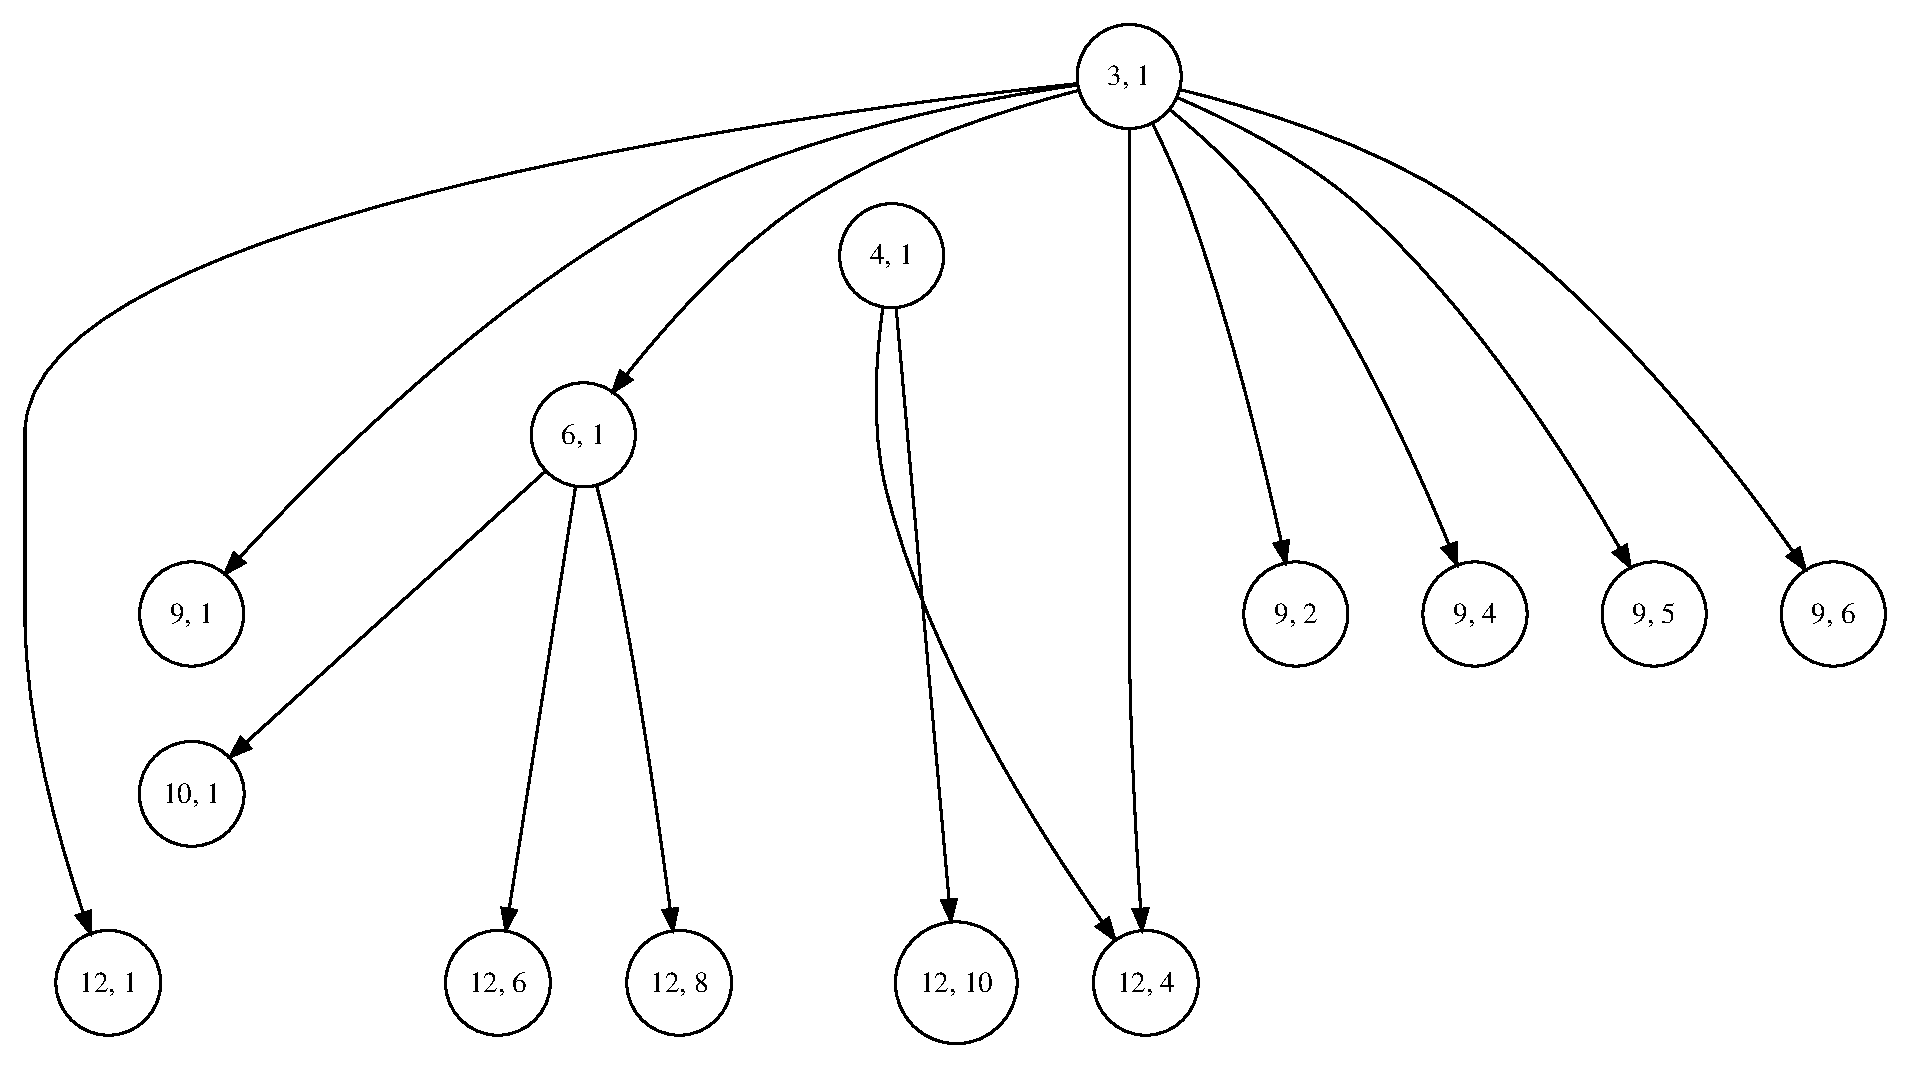
\includegraphics[scale = 0.4]{Thesis/images/SubQuandle1.eps}
    \caption{}
    \label{fig:subqgraph}
\end{figure}

\subsection{Visualising congruence lattices of left quasigroups}\textcolor{white}{line}\newline
\noindent The algorithms to compute the congruences of a left quasigroup available in \Software~can be used to draw the congruence lattice of any left quasigroup. The commutator theory for racks and quandles is described in \cite{BonStanCommTheory2021}, it is built on the commutator theory for universal algebra developed by Smith in \cite{smith1976varieties} and expanded by Freese in \cite{freese1987commutator}. 

Restricting the focus on racks, it is possible to distinguish whether a congruence $\sim$ on a rack $\algebra{A}$ is central, or abelian, according to group-theoretic properties of $\Dis_\sim(\algebra{A})$ \cite{BonStanCommTheory2021}. The action of a group $H$ is $\sim$\emph{-semiregular} for a congruence $\sim$ on a rack $\algebra{A} = (S, \cdot)$ if for every $h\in H$, if $h(x) = x$ then $h(y)=y$ for any two elements $x,y \in S$ such that $X\sim y$. The congruence $\sim$ is called \emph{central} if and only if the action of $\Dis(\algebra{A})$ is $\sim$-semiregular on $\algebra{A}$ and $\Dis_\sim(\algebra{A})$ is central in $\Dis(\algebra{A})$ \cite{BonStanCommTheory2021}. The congruence $\sim$ is called \emph{abelian} if and only if the action of $\Dis_\sim(\algebra{A})$ is $\sim$-semiregular on $\algebra{A}$ and $\Dis_\sim(\algebra{A})$ is abelian \cite{BonStanCommTheory2021}. 

Figure \ref{fig:conglattice} shows three possible congruence lattices of a locally strict simple quandle, one whose all proper subquandles are strictly simple \cite{bonatto2022connected}. The vertices coloured in gold (\textcolor{gold}{$\blacksquare$}) indicate that the congruence is central, the vertices coloured in light green (\textcolor{olivedrab1}{$\blacksquare$}) indicate that the congruence is abelian.

\begin{figure}[H]

\centering
\hspace{5.5em}\includegraphics[scale=0.9]{Thesis/images/Coloured3_1LatticeGraph.eps}\hspace{5em}
\includegraphics[scale=0.6]{Thesis/images/Coloured28_3LatticeGraph.eps}\hspace{7em}
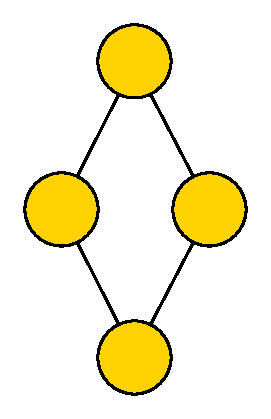
\includegraphics[scale=0.6]{Thesis/images/Coloured28_2LatticeGraph.eps}\hfill

\caption{(a) Simple (b) Subdirectly Irreducible (c) Subdirectly reducible}
\label{fig:conglattice}

\end{figure}
\noindent The following, more interesting, examples are the congruence lattices of the 10th connected quandle of order 36 and of the 42nd connected quandle of cardinality 36.
\begin{figure}[H]

\centering
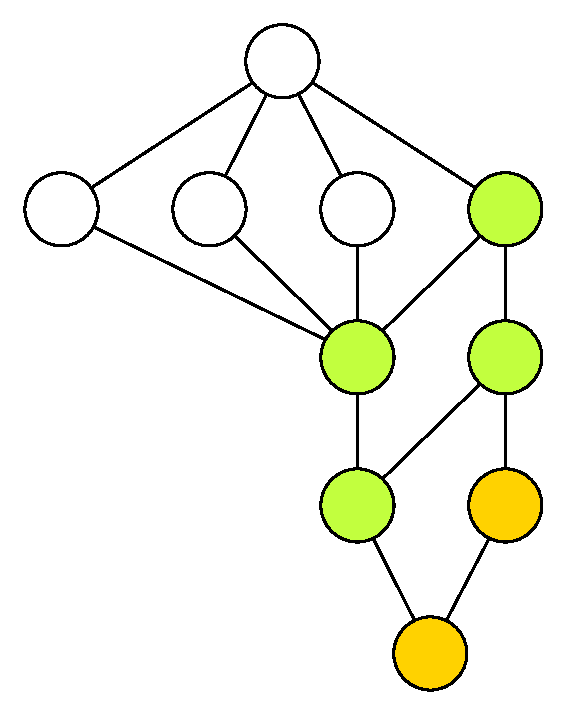
\includegraphics[scale=0.5]{Thesis/images/Coloured36_10LatticeGraph.eps}\hfill
\hfill\includegraphics[scale=0.5]{Thesis/images/Coloured36_42LatticeGraph.eps}\hfill

\caption{}


\end{figure}
\newpage\noindent The congruence lattice of a left quasigroup can convey information about the original structure. In the case of quandles, a congruence lattice as in Figure \ref{fig:conglattice}(c) indicates that the quandle is a direct product of a pair of quandles and congruence lattice as in Figure \ref{fig:conglattice}(b) might indicate a connected non-abelian locally strict simple quandle \cite{bonatto2022connected}.

\subsection{Visualising quotient structures}\textcolor{white}{line}\newline
\noindent Following this line of thought, one can visualise the factors of a quandle. \newline In Figure \ref{fig:qquandle}, one can see the graph of quotient quandles for all connected quandles up to order 12 where the vertex representing the quandle of order 1 was removed. The edges going from the quandles of greater order to those of smaller order are meant to represent the epimorphisms going from structure to quotient structure.
\begin{figure}[H]
    \centering
    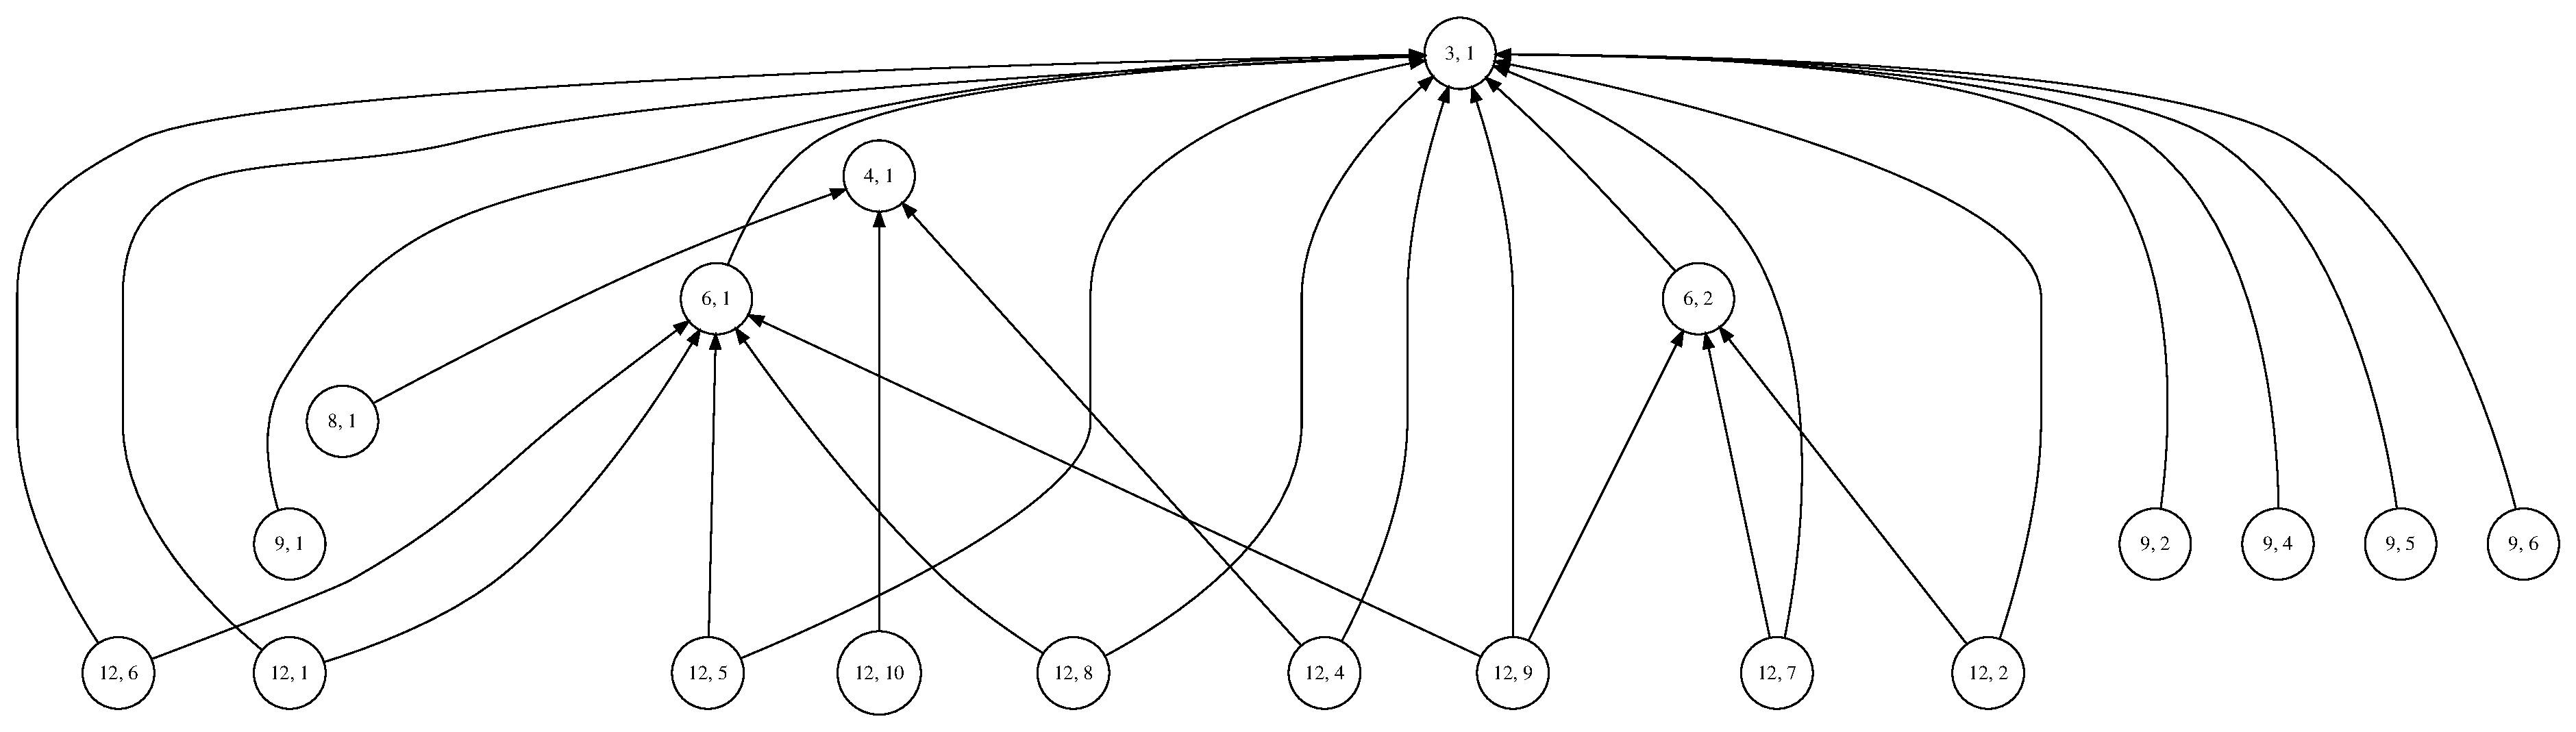
\includegraphics[scale = 0.25, angle=90]{Thesis/images/BigConnectedQuoQuandle.eps}
    \caption{}
    \label{fig:qquandle}
\end{figure}
\section{Comparison}
\noindent This section will show a comparison between \Software, \rig~and \cream~in terms of running times on the following tasks:  computation of the automorphisms group, search of a generating set, search of all subalgebras, computation of all congruences.

Each command has been run on a shared university terminal running Ubuntu 20.04.4 LTS (Focal Fossa) with AMD EPYC 7502P 32-Core Processor and a 64GB RAM. The algorithms have been tested on the full database of 791 connected quandles available in \rig. The values displayed are the medians: the median time taken by the software to carry out the tasks mentioned above for a connected quandle of order $x\in [X,Y]\subset \mathbb{N}$.\newline 
The author decided to display the median instead of the traditional mean because, due to a few peculiar quandles in the database, the results would not have reflected the time taken to carry out the tasks mentioned above for most connected quandles, they would have been heavily skewed towards high untruthful values. 



\begin{table}[H]
    \label{genSetTable}
    \centering
    \begin{tabular}{|c|c|c|c|}
        \hline
         Order & \textsf{QuandleRUN}(s) & \textsc{Rig}(s) & \textsc{CREAM}(s) \\ \hline
         1-10 & 0.000 & 0.000 &  0.000\\ \hline
         11-20 & 0.000 & 0.001 &  0.002\\ \hline
         21-30 & 0.000 & 0.004 & 0.004 \\ \hline
         31-40 & 0.000 & 0.007\footnotemark[1]  & 0.006  \\ \hline
         41-47 & 0.000 & \ding{55} & 0.009  \\ \hline
    \end{tabular}
    \caption{Running times to find a generating set.}
    
\end{table}
\footnotetext[1]{The computation was interrupted while working on the last quandle of order 36; it reached the pre-set memory limit.}

\noindent According to \hyperref[genSetTable]{Table 1}, when finding a generating set, \cream~is very fast but slightly slower than \Software. This is due to the fact that \Software~skips the computation of invariants, \emph{and} the computations of subalgebras generated by one element by explointing the idempotence of quandles.
\rig~is slower than both because first it computes all the subsets of the underlying set of the quandle of cardinality 1 and checks whether any of them generates the quandle; if not, it moves to all the subsets of cardinality 2 and checks whether any of them generates the quandle and so on until a generating set is found.

\begin{table}[H]

    \centering
    \begin{tabular}{|c|c|c|c|}
        \hline
         Order & \textsf{QuandleRUN}(s) & \textsc{Rig}(s) & \textsc{CREAM}(s) \\ \hline
         1-10 & 0.000 & 0.000 & 0.001 \\ \hline
         11-20 & 0.020 & 0.022 & 0.003 \\ \hline
         21-30 & 0.060 & &  0.007 \\ \hline
         31-40 & 0.165 & & 0.011  \\ \hline
         41-47 & 0.300 & & 0.016 \\ \hline
    \end{tabular}
    
    \caption{Running times to compute the automorphism group.}
    \label{AutTable}
\end{table}
\noindent According to \hyperref[AutTable]{Table 2}, which refers to the computation of the automorphism group, one can see that, while \Software~is faster than \rig, the only software available explicitly dedicated to the study of quandles, \cream~is definitely the winner of this competition. This is interesting since the strategies used by \rig~and \cream~are very similar and the only differences between them are that \cream~looks for a generating set before looking for the automorphisms, since that might reduce the number of trials necessary to find valid homomorphisms, as explained in \hyperref[monomorphismAlgo]{Section 3.1.3}. Furthermore, most of the computation of \cream~is written in the programming language \texttt{C} rather than the language of the computer algebra system \textsc{GAP}.
\rig~naïvely tries to assign different images to the values of the domain until all valid automorphisms have been found. The use of \texttt{C}, combined with a different strategy, on the other hand, explains the advantage of \cream~over \Software.
 
\begin{table}[H]
    \label{subTable}
    \centering
    \begin{tabular}{|c|c|c|c|}
        \hline
         Order & \textsf{QuandleRUN}(s) & \textsc{Rig}(s) & \textsc{CREAM}(s) \\ \hline
         1-10 & 0.000 & 0.000 & 0.001 \\ \hline
         11-20 & 0.001 & 0.006 & 0.005 \\ \hline
         21-30 & 0.005 & 0.042 & 0.016 \\ \hline%0.165quandlerun
         31-40 & 0.170 & 0.149 &   \\ \hline
         41-47 & 0.250& 0.316&    \\ \hline
    \end{tabular}
    \caption{Running times to find all subalgebras.}
\end{table}
 \noindent According to \hyperref[subTable]{Table 3}, \Software~and \rig~are the winners when computing subalgebras. \cream~needs to compute the automorphisms group first and then, for any subalgebras it finds ``naïvely", it applies the action of the automorphisms group to find all the other ones generated by the same amount of generators until it can only find the underlying set of the superquandle. \cream~is very fast in computing the set of automorphisms (as can be seen above) but it applies the automorphisms naïvely and does not use hash tables to check whether it has already seen a quandle or not. These are all contributing factors that make it the slowest of the three in the long run, while \rig, with its simplicity, manages to almost keep up with \Software~and even be much faster in a handful of instances. For example, computing all the subalgebras of the $45$th quandle of order $45$ in \Software~takes over $8$ hours whereas \rig~needs slightly less than 3 hours. This advantage might be explained, in minimal part, by technical differences of the underlying systems, \textsc{GAP}~and \magma: \textsc{GAP} allows the user to add elements to the list at the base of a for-loop whereas, in \magma, once a for-loop over a list is defined, elements can be added to the list but the for loop will stop once it reaches the elements that was the last element when the for loop was defined. This means that to achieve a similar behaviour, \Software~has to use a while loop that needs to check the loop condition at each iteration which slows the process down.
\begin{table}[H]
    \centering
    \begin{tabular}{|c|c|c|}
        \hline
         Order & \textsf{QuandleRUN}(s) & \textsc{CREAM}(s) \\ \hline
          1-10 & 0.000 & 0.000 \\ \hline
         11-20 & 0.000 & 0.000 \\ \hline
         21-30 & 0.000 & 0.002\\ \hline
         31-40 & 0.000 & 0.007\\ \hline
         41-47 & 0.000 & 0.013 \\ \hline
    \end{tabular}
    \caption{Running times to compute all congruences}
    
\end{table}
\noindent Finally, the system are compared based on how they perform when computing all congruences. \rig~cannot compute the congruences of a quandle. The difference in speed between \Software~and \cream~can be explained by the difference in strategy. \Software~relies on \magma~to constructs all non-trivial partitions preserved by the left multiplication group of the connected quandle. This ensures speed, since \Software~will only need to check the second condition of Lemma \ref{lemma1.5medial}, and guarantees that \Software~will not have to deal with possible duplicates. \cream, on the other hand, needs to unarify the algebra, construct the congruences ``manually" and make sure that there are no duplicates which takes time.
% \chapter{Related Work}\label{relatedwork}
In this chapter you demonstrate that you are sufficiently aware of the
state-of-art knowledge of the problem domain that you have investigated as
well as demonstrating that you have found a \emph{new} solution / approach / method.

\chapter{Conclusions}\label{conclusions}
\noindent This document aimed to introduce \Software, a modern tool for research in the theory of quandles. It shows how, by incorporating existing ideas, developing new ones based on recently discovered theory, or by looking at the theory from a different perspective, one can provide the foundations for an open and easily extendable research tool. Furthermore, being fully written in \magma, it ensures that researchers have at their disposal the best instruments to improve upon it.

Just like \magma, \Software~uses the language of sets and maps and, thus provides a natural way to any mathematician of describing computations both to improve their own tool or to explore new ideas in quandle theory. Furthermore, \Software~provides a common language for quandle theorists and a common interface to a library of algorithms; all things bound to improve communication and favour computational experimentation. This document hopes to stimulate a more experimental way of researching and hopes that \Software~can be a tool that, quoting \cite{borwein2004experimentation}:
\begin{quote}
    \emph{``[...] provides a compelling way to generate understanding and insight; to generate and confirm or confront conjectures; and generally to make mathematics[Author's note: read \textit{Quandle theory} here] more tangible, lively, and fun for both the professional researcher and the novice."}
\end{quote}
The source code of \Software~along with the examples of \hyperref[AppSection]{Section 4} can be found on \underline{\href{https://github.com/Ingolfurinn/QuandleRUN-Thesis}{GitHub}}.
\section{Future Direction \& Open Problems}
\begin{itemize}
    \item Adapt \cite{atkinson} or \cite{schonert1994finding} to work on non-transitive groups. This would make Algorithm \ref{congsSmart1} work on any left quasigroup.
    \item Attempt to define the theoretical complexity of Algorithms \ref{congsSmart1} and \ref{congsSmart2} and compare it with Algorithm \ref{congsFreese}.
    \item In order to make algorithms such as Algorithm \ref{quandlerunSubs} faster, hashing functions with better collision rates for sets of integers are needed. 
    \item Ways to reduce the search space for automorphisms of a left quasigroup are needed, this would make Algorithm \ref{qrunauto} even faster.
    \item Implement \texttt{LeftTransversal($G$, $H$)} mentioned in Algorithm \ref{alg:coset}, to make the construction of coset quandles faster. 
\end{itemize}



% \bibliographystyle{plain}
\bibliographystyle{acm}
\bibliography{bibliography}

% \appendix
% \input{appendix}

\end{document}
